% https://home.hirosaki-u.ac.jp/masumi/100/
\documentclass[a4paper,12pt]{jsarticle}
% \documentclass[a4paper]{jsarticle}
\usepackage{bm}
\usepackage[dvipdfmx]{graphicx}
\usepackage{ascmac}
\usepackage{amsmath}
% bibtex use natbib.sty
% https://www.imperial.ac.uk/media/imperial-college/administration-and-support-services/library/public/LaTeX-example-Harvard-apr-2019.pdf
\usepackage{natbib}
% argmin定義
\DeclareMathOperator*{\argmin}{arg\,min}
% ハイパーリンク
\usepackage[dvipdfmx]{hyperref}
\usepackage{pxjahyper}
\usepackage{booktabs}
% 表を横に
\usepackage{lscape}
% 表の脚注
% https://qiita.com/kumamupooh/items/38795811fc6b934a950d
\usepackage{threeparttable}
% 表のセル内改行
% \usepackage{tabularx}
% \usepackage{array}
% \newcolumntype{C}[1]{>{\centering\arraybackslash}p{#1}}
% 番号付き箇条書き
\usepackage{enumerate}
% サブキャプション入り図を並べて表示
% https://atatat.hatenablog.com/entry/cloud_latex18_subcaption
\usepackage[hang,small,bf]{caption}
\usepackage[subrefformat=parens]{subcaption}
\captionsetup{compatibility=false}
% 図のfootnote
\usepackage[capposition=top]{floatrow}

\hypersetup{
setpagesize=false,
 bookmarksnumbered=true,%
 bookmarksopen=true,%
 colorlinks=true,%
 linkcolor=black,
 citecolor=black,
}

\title{機械学習アルゴリズムによる\\
  日本企業の四半期利益予測}
\author{早稲田大学大学院商学研究科 商学専攻\\
  35201064 王思涵}
% \date{2021年月日}

\begin{document}
\maketitle
\tableofcontents

\part{はじめに}

1株当たり利益(Earnings Per Share: EPS)は,企業の当期純利益を発行株式数で割ったものであり,規模に依存しない企業の収益性を捉えた指標である.企業外部のステークホルダーである投資家は,企業の将来のEPSの予測をもとに,収益性の高いポートフォリオを構築したり,将来の株価収益率を算出して投資判断を行う.また,企業内部の経営者は将来のEPSの予測を用いて,営業予算の作成や設備投資の判断などの重要な意思決定を行う.したがって,EPSを正しく予測することは企業内外の幅広いステークホルダーにとって重要である.

企業の将来利益の予測は,人的な予測と,統計的・機械的な予測の2つに大別できる\citep{sakurai1990}.人的な予測の代表として,アナリスト予測がある.アナリスト予測とは,株式市場分析の専門家である証券アナリストが公表する利益予測である.他方,統計的・機械的な予測とは,過去の実績データをもとに何らかの時系列モデルを用いて将来の利益を予測するものである.モデルに基づく予測は,予測値を導出するまでの過程を全て自動化できるため,人的な予測に比べてコストが低いという特徴を有している\citep{sakurai1990}.

統計的・機械的な予測に関する研究で用いられているモデルは,1)「単変量」か「多変量」か,2)「線形」か「非線形」か,の2つの観点で分類できる\citep{zhang2004neural}.従来の,モデルに基づくEPS予測の研究の多くは,自己回帰和分移動平均(AutoRegressive Integrated Moving Average: ARIMA)モデル\citep*{box2015time}などの単変量で線形な統計的時系列モデルを用いている\citep*{foster1977quarterly, griffin1977time, brown1979univariate}.一方,近年の研究では,「ファンダメンタル会計変数(Fundamental accounting variables)」を用いた多変量モデルによるEPS予測の研究が増えている.ファンダメンタル会計変数とは,売掛金,棚卸資産,資本的支出といったいくつかの会計変数のことであり,これらの変数には将来のEPSを予測する情報があるとされている\citep*{lev1993fundamental, abarbanell1997fundamental}.また,四半期EPSデータには非線形性があるとされており\citep*{hopwood1986univariate},これを考慮するために,予測モデルに非線形性を反映させている研究も盛んである.中でも従来の統計的時系列モデルに代替されるモデルとして,機械学習アルゴリズムが注目されている.機械学習アルゴリズムには,従来の統計的時系列モデルに比べて,高次元データの処理に長けたモデルや非線形性を捉えられるモデルが豊富にある\citep*{cao2020fundamental}.そのため機械学習アルゴリズムを用いることで,多変量なファンダメンタル会計変数から予測情報を抽出し,企業利益データの非線形性を捉え,精度の高いEPS予測が得られると考えられる.

機械学習アルゴリズムによるEPS予測の研究は多くの国の企業を対象として行われている.\cite{zhang2004neural}はアメリカのニューヨーク証券取引所の上場企業,\cite*{cao2009forecasting} は中国の上海証券取引所と深セン証券取引所の上場企業,\cite{etemadi2015earnings}はイランのテヘラン証券取引所の上場企業を対象に,機械学習アルゴリズムの1つであるNNによる四半期EPSの予測を行っている.また,\cite*{cao2020fundamental}はアメリカの上場企業を対象に,いくつかの代表的な機械学習アルゴリズムを用いた年次EPS予測を行っている.いずれの研究においても機械学習アルゴリズムが精度の高い予測を与える結果となっている.

このように近年,統計的・機械的な手法によるEPS予測の研究分野では,機械学習アルゴリズムを用いることで予測の精度が向上することが様々な国のサンプルで確認されている.しかし,\cite{ota2006}によると日本における人的な予測と従来の時系列モデル予測の精度比較研究については,明確な結論が出ていないにも拘らず,モデルによる予測よりも人的な予測の方が適切であると暗黙裡に見なされており,時系列モデルによる予測の研究は,現在では衰退している.現に日本における統計的・機械的なEPS予測の研究は限定的で従来の線形時系列モデルの適用に留まっており,高い予測精度が期待される機械学習アルゴリズムを用いた日本企業を対象とするEPS予測の研究は,筆者の知る限り存在しない.また,日本では時系列モデルによる利益予測が衰退したあとの2008年度に四半期報告制度が創設されているため,四半期データを用いたEPS予測の研究もない.

そこで,日本企業データにおいて、機械学習アルゴリズムは、従来の統計的時系列モデルに比べEPS予測の精度を向上させるのか,人的な予測よりも高い精度の予測を与えるのかを検証することを本稿の目的とする.具体的には東京証券取引所一部上場企業を対象に機械学習アルゴリズムによる四半期EPS予測を行い,得られた予測値を用いて従来の線形時系列モデルによる予測やアナリストによる予測と精度比較をする.追加的な検証として,各手法による予測値それぞれに基づいた株価予想利益率からロング・ショートポートフォリオを構築し,それを日本の証券市場に適用させて,機械学習アルゴリズムによる予測の投資指標としての有用性を考察する.

本稿の構成は次のとおりである.まず第\ref{par:litrev}部では過去のEPS予測に関する研究や機械学習アルゴリズムを用いた時系列予測に関する研究について紹介する.次に第\ref{par:data},\ref{par:model}部で本稿で用いるデータ及び予測モデルについて説明し,第\ref{par:result}部で本稿の予測結果について報告する.第\ref{par:portfolio}部では追加的な検証を行い,最後に 第\ref{par:conclusion}で本稿の結論を述べる.

\part{過去の研究} \label{par:litrev}

これまで多くの企業利益予測の研究で,統計的・機械的な予測手法間の精度比較,統計的・機械的な予測手法と人的な予測手法の精度比較,人的な予測手法間の精度比較が行われている.\cite{sakurai1990}や\cite{ota2006}のレビュー論文は,そのような数々の利益予測の研究に関する文献についてまとめている.アメリカの利益予測の研究に関して,\cite{sakurai1990}は以下のようにまとめている.<ーーまずEPSを予測する伝統的な時系列モデルについて,年次EPSはランダムウォークによってうまく描写され,四半期EPSは\cite*{brown1979univariate},\cite{griffin1977time},\cite{foster1977quarterly}の3つのARIMAモデルによってうまく描写されると述べている.一方で,アナリスト予測と伝統的な時系列モデルによる予測の比較については,アナリストによる年次および四半期のEPS予測が伝統的な時系列モデルによる予測よりも正確であると述べている.その理由として,アナリストは広く最新な情報集合を予測に用いるからである.ーー><ーー\cite{ota2006}は,日本の利益予測に関する研究はそれほど盛んではないが、比較結果はアメリカのものと同様であることを指摘している。ーー><ーーそして,日本の時系列モデルによる利益予測については,「アナリスト予測との精度比較の明確な結論が出ていないにも拘わらず,最近の研究では時系列モデルによる予測よりもアナリスト予測を用いる方が市場の期待利益として適切であると暗黙裡に見なされており,時系列モデルによる利益予測の研究は,現在では衰退している」と述べている.ーー>

ここで注意するべき点として,上記で言及されている利益予測精度の比較の研究で扱われている時系列モデルの多くは,あくまでも当時研究が盛んであった伝統的な単変量で線形の時系列モデルのことであり,代替的な多変量モデルや非線形モデルについては議論されていない.\cite{ota2006}は「ナイーブな時系列を用いた場合には人的な予測の方が精度が高いが,高度な時系列モデルを用いた場合には時系列モデルの予測の方が人的な予測よりも精度が高いといえる」と述べており,モデルを発展させることで統計的・機械的なEPS予測の精度は向上する余地があることを示唆している.

近年,多くの学術分野で応用され成果を上げている予測モデルとして,機械学習アルゴリズムの1つであるニューラルネットワーク(Neural Network: NN)モデルが挙げられる.NNは生物の神経細胞(ニューロン)の構造と機能をもとに考案された数学モデルであり,従来の統計モデルに比べて非線形で不定形な問題にうまく対処できることから,多数の分野での利用が増加している\citep*{tkavc2016artificial}.特に,\cite{hill1996neural}は,月次や四半期の時系列データにおいてNNの方が伝統的な統計モデルよりも正確な予測を与えるとし,時系列予測におけるNNの有用性を示している.その理由として,NNはあらゆる関数形を近似できる普遍性定理(Universal Approximation Theorem)\citep{hornik1989multilayer}により,伝統的な線形時系列モデルでは捉えられない時系列データの非線形性を捉え,予測モデルの関数形の誤特定を回避できるからであると述べている.また,\cite{hill1994artificial}は,予測の対象である時系列データが,i)財務的,ii)季節的,iii)非線形な特徴を有するとき,NNによる予測は従来の線形時系列モデルよりも精度が高い傾向があると述べている.特に四半期EPSは,上記の3つの特徴を有することが確認されている\citep*{hopwood1986univariate}.

そこで,\cite{callen1996neural}はニューヨーク株式市場の企業を対象に,単変量の四半期EPS予測におけるNNと従来の統計的手法であるARIMAモデルとの精度比較を行ったが,結果は予想に反してNNの予測精度がARIMAモデルに比べて低いものとなっている.そして,この研究ではNNの予測精度は文脈依存であると結論付けている.
% (Hillのディスポイント)

一方,会計学の研究では,企業利益の予測について,将来の利益を説明する変数を特定することに注目してきた.\cite*{lev1993fundamental}は,アナリストが有価証券の価値評価において有用であるとされる会計変数を調査し,それらの会計変数が将来の企業利益と関連があると述べている.言及された会計変数は以下のとおりである.

\begin{itemize}
\item 棚卸資産 (Inventories) \\
    売上原価の増加に対して過度な棚卸資産の増加は,売上高を増加させることが困難であることを示唆するため,ネガティブなシグナルとみなされる.さらに,棚卸資産が増加すると経営者は在庫を減らそうとするため,将来の利益が減少するシグナルになり得る.

\item 売掛金 (Accounts receivable) \\
    売上高に対して過度な売掛金の増加は,企業の製品販売が困難な状態にあることや,賃倒引当金の増加などを意味し,将来の利益が減少するシグナルになり得る.

\item 資本的支出 (Capital expenditures) \\
    資本的支出の過度な減少は,以前の投資水準を維持するための現在および将来のキャッシュフローが十分でないという経営者の懸念を意味する.このように一般的に資本的支出の減少は,短期的な経営志向とみなされ,将来の利益が減少するシグナルになり得る.

\item 売上総利益 (Gross margin) \\
    売上総利益は企業の競争の激しさや営業レバレッジなどの要因を捉え,これが企業の長期的なパフォーマンスに影響を与える.したがって,売上総利益は企業の利益の持続性や企業価値に関して有益な情報をもち,売上高に対して過度な売上総利益の減少は,将来の利益が減少するシグナルになり得る.

\item 販売費および一般管理費 (Selling and administrative expenses) \\
    ほとんどの場合,販売費および一般管理費は一定であるため,売上高に対して過度な販売費および一般管理費の増加は,コストコントロールの喪失や異常な販売努力を示唆し,将来の利益が減少するシグナルになり得る.

\item 実効税率 (Effective tax rate) \\
    法定税率の変更に依らない企業の実効税率の大幅な変化は,一般的には一時的なものとして捉えられる.したがって,過度な実効税率の低下は将来の利益が減少するシグナルになり得る.

\item 労働力 (Labor force) \\
    一般的に労働力の削減の発表に対してアナリストは好意的な反応を示す.したがって,過度な労働力の増加は将来の利益が減少するシグナルになり得る.
\end{itemize}

\cite*{abarbanell1997fundamental}では,上記の会計変数をファンダメンタル会計変数とし,ファンダメンタル会計変数が将来のEPSの変化を説明するかどうかについて検証している.分析の結果,ファンダメンタル会計変数と将来のEPSの変化の間に強い関係が確認され,ファンダメンタル会計変数に含まれる会計情報は,将来のEPSに対して予測能力を持つと述べている.

これを受け\cite{zhang2004neural}は,\cite{callen1996neural}の単変量NNによる四半期EPS予測の研究を発展させる形で,NNにファンダメンタル会計変数を反映させた多変量NNによる四半期EPS予測を行った.この研究では,単変量線形モデル,多変量線形モデル,単変量NN,多変量NNの4つのカテゴリー間で精度比較を行っており,結果として,NNは線形モデルよりもうまくファンダメンタル会計変数の情報を反映し,より精度の高いEPSの予測値を与えた.その後,様々な国のサンプルでEPS予測におけるNNの有用性を示した研究が行われている.\cite*{cao2009forecasting} は中国の上海証券取引所と深セン証券取引所の上場企業,\cite{etemadi2015earnings}はイランのテヘラン証券取引所の上場企業を対象に,ファンダメンタル会計変数を反映させたNNによるEPS予測を行っており,いずれも高い精度の予測を与える結果を得ている.

このように近年の四半期EPS予測の研究では多変量NNが盛んに用いられているが,機械学習アルゴリズムの1つであるNNだけが注目されており,他の機械学習アルゴリズムを用いた研究は限られている.これはEPS予測の文脈に限らず,他の時系列予測研究でもNNのみに着目している傾向がある\citep{ahmed2010empirical}.しかし,NN以外の機械学習アルゴリズムが四半期EPS予測において成果を上げられる可能性も十分にある.代表的な機械学習アルゴリズムとして,罰則回帰モデルやランダムフォレスト回帰が挙げられる\citep{hastie2009esl}.罰則回帰モデルは,高次元データに対して変数選択・係数縮小を行うことで多数の説明変数から目的変数を予測する情報を抽出し,精度の高い予測を行うことができるため,四半期EPSの多変量予測において有用であると考えられる.また,ノンパラメトリックで非線形なランダムフォレスト回帰\citep{breiman2001random}も,NNとは異なったアルゴリズムで四半期EPSデータの非線形性を捉えることができると考えられる.<ーー\cite*{cao2020fundamental}は年次であるものの,これらの代表的な機械学習アルゴリズムを用いたEPS予測を行っており,ベンチマークであるランダムウォークよりも精度の高い予測を与える結果を報告している.ーー>

% (Hill et al のNNディスも少し入れる)

以上の過去の研究を踏まえ,現状の日本のEPS予測における「時系列モデルが古典的な手法にとどまっていること」と「時系列モデルと人的な予測の優劣の曖昧さ」の2つの課題に対し,本稿は機械学習アルゴリズム(NN,罰則回帰モデル,ランダムフォレスト回帰)にファンダメンタル会計変数を含めて日本企業の四半期EPS予測を行い,さらに時系列モデルとアナリストのEPS予測精度を比較し,予測手法間の精度の優劣を明らかにする.

\part{データ} \label{par:data}

\section{サンプルデータ} \label{sec:sample}

日本の四半期報告制度は比較的新しく,2007年の企業会計基準委員会(ASBJ)による企業会計基準第12号「四半期財務諸表に関する会計基準」及び企業会計基準適用指針第14号「四半期財務諸表に関する会計基準の適用指針」の公表以降,上場企業の四半期報告書の提出が義務付けられた.\footnote{2011年に企業会計基準委員会(ASBJ)は改正企業会計基準第12号「四半期財務諸表に関する会計基準」及び改正企業会計基準適用指針第14号「四半期財務諸表に関する会計基準の適用指針」等の公表をしている.この四半期報告制度の改正では財務諸表作成者の作成負担を考慮し,いくつかの四半期情報の開示を義務ではなく任意とされている.それに伴い,四半期報告制度の改正以降,資本的支出と期末従業員数の観測される頻度が減り,欠損が多く見られる.\cite{zhang2004neural}は四半期単位で欠損している資本的支出と期末従業員数について,資本的支出は毎四半期均等であるとし,期末従業員数は前期の値を維持すると仮定して,欠損値を補填している.本稿でもこの方法に倣って資本的支出と期末従業員数の欠損処理を行うこととする.}

これにより,四半期データを分析の単位とする本稿では,サンプル期間を四半期報告制度が適用された2008年度(2008年4月1日)から現在2020年度(2021年3月31日)までの計52四半期とする.また,本稿の分析対象企業(サンプル企業)を,サンプル期間において以下の基準で選択する.

\begin{itemize}
  \item 東京証券取引所一部上場企業
  \item 3月決算企業
  \item 一般事業者(「銀行業」,「証券,商品先物取引業」,「保険業」,「その他金融業」を除く)
  \item 各四半期の中間月末(5月末,8月末,11月末,2月末)までに前四半期決算を発表している企業\footnote{IBES予測及びポートフォリオ構築のタイミングをそろえるため.}
\end{itemize}

四半期EPS(3ヶ月)およびファンダメンタル会計変数の算出に必要な四半期会計データは「日経NEEDS-FinancialQUEST」から収集している.結果,1,003社,延べ $1,003社 \times 52四半期 = 52,156個$の企業四半期が最終サンプルである.表\ref{tab:ind}はサンプル企業の業種別の内訳を示している.なお,所属業種は証券コード協議会の中分類(全33種)に基づいている.

\begin{table}
  \centering
  \caption{業種(証券コード協議会中分類33種)}
  \label{tab:ind}
  \scalebox{0.7}[0.7]{
    \begin{threeparttable}  

\begin{tabular}{llr}
\toprule
{} &       業種名 &  企業数 \\
業種コード &           &      \\
\midrule
3650  &      電気機器 &  108 \\
6050  &       卸売業 &  101 \\
3200  &        化学 &   92 \\
3600  &        機械 &   83 \\
2050  &       建設業 &   70 \\
5250  &    情報・通信業 &   66 \\
9050  &     サービス業 &   59 \\
6100  &       小売業 &   54 \\
3050  &       食料品 &   44 \\
3700  &     輸送用機器 &   41 \\
5050  &       陸運業 &   34 \\
3450  &        鉄鋼 &   28 \\
3800  &     その他製品 &   27 \\
3100  &      繊維製品 &   24 \\
3400  &  ガラス・土石製品 &   23 \\
3250  &       医薬品 &   23 \\
3550  &      金属製品 &   22 \\
3750  &      精密機器 &   20 \\
8050  &      不動産業 &   19 \\
3500  &      非鉄金属 &   14 \\
5200  &  倉庫・運輸関連業 &   12 \\
3150  &     パルプ・紙 &    8 \\
5100  &       海運業 &    7 \\
4050  &    電気・ガス業 &    7 \\
3300  &   石油・石炭製品 &    5 \\
3350  &      ゴム製品 &    4 \\
0050  &    水産・農林業 &    3 \\
1050  &        鉱業 &    3 \\
5150  &       空運業 &    2 \\ \cline{2-3}
      &         合計 & 1,003 \\
\bottomrule
\end{tabular}

\begin{tablenotes}
      \item[](出所)筆者作成.
\end{tablenotes}
\end{threeparttable}  
  }
\end{table}

\section{目的変数}

予測の対象となる四半期1株あたり利益(四半期EPS)は以下のように定義される.

\begin{equation}
  \begin{split}
    Y &= \text{四半期 1株あたり利益} \\
    &= \frac{普通株式に係る四半期当期純利益}{普通株式の期中加重平均株式数} \\
    &= \frac{損益計算書上の四半期当期純利益-普通株式に帰属しない金額}{普通株式の期中加重平均発行済株式数 - 普通株式の期中加重平均自己株式数} \\  
  \end{split}
\end{equation}

\section{説明変数}

単変量モデルによる四半期EPS予測は,過去の四半期EPSの実績値のみを説明変数として用いる.一方,多変量モデルによって四半期EPSを予測する場合は,過去の四半期EPSに加えて,\cite{lev1993fundamental}や\cite{abarbanell1997fundamental}が企業の将来のEPSに対して予測能力を持つと言及しているファンダメンタル会計変数も説明変数として用いる.本稿では,ファンダメンタル会計変数を実際に四半期EPS予測に用いた\cite{zhang2004neural}に倣って以下のように7つのファンダメンタル会計変数を定義する.

\begin{equation}
  \begin{split}
    INV &= \frac{棚卸資産(円)}{普通株式の期中加重平均株式数} \\
    AR &= \frac{売掛金(円)}{普通株式の期中加重平均株式数} \\
    CAPX &= \frac{資本的支出(円)}{普通株式の期中加重平均株式数} \\
    GM &= \frac{売上総利益(円)}{普通株式の期中加重平均株式数} \\
    SA &= \frac{販売費及び一般管理費(円)}{普通株式の期中加重平均株式数} \\
    ETR &= \frac{法人税(円)}{税引前利益(円)} \\
    LF &= \log{\left(\frac{売上高(円)}{従業員数(人)}\right)} \\
  \end{split}
\end{equation}

% 多変量モデルによる予測では四半期EPSとファンダメンタル会計変数の4期までのラグを説明変数として用いる.
表\ref{tab:summary}は予測に用いる変数の記述統計を示している.

\begin{table}
  \centering
  \caption{変数の記述統計量}
  \label{tab:summary}
  \scalebox{0.7}[0.7]{
    \begin{threeparttable}  

\begin{tabular}{lrrrrrrrr}
\toprule
{} &        Y &         INV &          AR &        CAPX &          GM &         SA &        ETR &         LF \\
\midrule
count &  52,156 &   52,156 &   52,156 &   52,156 &   52,156 &  52,156 &  52,156 &  52,156 \\
mean  &     67.468 &     808.786 &    1272.915 &     173.152 &     513.363 &    385.510 &      0.339 &     16.205 \\
std   &    707.529 &    7,234.778 &    8,087.579 &    2,387.784 &    3,577.896 &   2,699.862 &      5.835 &      0.793 \\
min   & -37,300.500 &       0.011 &       0.026 &       0.001 &  -30,368.482 &   -482.938 &   -494.716 &     11.628 \\
25\%   &      3.490 &      91.615 &     181.897 &       9.296 &      53.156 &     39.603 &      0.241 &     15.662 \\
50\%   &     15.230 &     193.908 &     357.978 &      24.741 &     115.768 &     83.523 &      0.331 &     16.154 \\
75\%   &     37.540 &     415.649 &     717.761 &      64.527 &     222.790 &    166.317 &      0.414 &     16.693 \\
max   &  31,202.830 &  404,482.462 &  293,004.896 &  143,224.390 &  104,813.930 &  87,333.561 &    817.750 &     22.531 \\
\bottomrule
\end{tabular}

\begin{tablenotes}
    \item[](出所)筆者作成.
\end{tablenotes}
\end{threeparttable}  
  }
\end{table}

% GM,SA,ETRが負になる説明
    
\part{予測モデル} \label{par:model}

\section{予測のデザイン}

本稿では,サンプル企業1,003社について,それぞれ1社ごとに1四半期先予測を12期(3年)分行う.まず,ある企業の全52四半期サンプル期間\footnote{実際のモデル推定では説明変数にラグ変数を含める.したがって利用できるサンプル期間は$52 - ラグの次数$である.モデルのデザインによってラグの次数は異なるため,利用できる訓練データの長さもモデルによって異なる.}をもとに,1つあたり長さ41期のローリングサンプル(rolling sample)を12個形成する.次に,1つのローリングサンプルを,過去40期の訓練データ(training data,in-sample)と最新1期のテストデータ(test data,out-of-sample)に分ける.そして訓練データを用いてモデルを推定し,テストデータと同じ期にあたる1期先の予測を行う.これを12個のローリングサンプルで繰り返すことによって,ある企業の1四半期先予測が12期分得られる.

つまり具体的には,ある企業の全52四半期サンプル期間 $\left\{Data_{\text{2008Q1}}, Data_{\text{2008Q2}}, \cdots, Data_{\text{2020Q4}}\right\}$ から12個のローリングサンプルを作り,1つ目の長さ41期のローリングサンプル $\{Data_{\text{2008Q1}}, Data_{\text{2008Q2}},$ $\cdots, Data_{\text{2017Q4}}, Data_{\text{2018Q1}}\}$ を長さ40期の訓練データ $\left\{Data_{\text{2008Q1}}, Data_{\text{2008Q2}}, \cdots, Data_{\text{2017Q4}}\right\}$ と長さ1期のテストデータ $\left\{Data_{\text{2018Q1}}\right\}$ に分ける.そして訓練データを用いてモデルを推定したあと,テストデータの説明変数をモデルに代入して訓練データの1期先の四半期EPS,$Y_{2018Q1}$ の予測値 $\hat{Y}_{2018Q1}$ を求める.2つ目のローリングサンプル $\left\{Data_{\text{2008Q2}}, Data_{\text{2008Q3}}, \cdots, Data_{\text{2018Q1}}, Data_{\text{2018Q2}}\right\}$ も同様に 訓練データ $\left\{Data_{\text{2008Q2}}, Data_{\text{2008Q3}}, \cdots, Data_{\text{2018Q1}}\right\}$ を用いて1期先の四半期EPSの予測値 $\hat{Y}_{2018Q2}$ を求める.同様に他のローリングサンプルに対しても,それぞれ同じモデルを異なる期間の訓練データで推定することで,1企業につき予測期間は2018年度第1四半期~2020年度第4四半期の12期となり,1四半期先予測値系列 $\left\{\hat{Y}_{2018Q1}, \hat{Y}_{2018Q2}, \cdots, \hat{Y}_{2020Q4}\right\}$ が得られる.この予測プロセスを全サンプル企業1,003社に対して行うことで,最終的に$12期 \times 1,003社 = 12,036個$の四半期EPS予測値が各予測手法から算出される.図\ref{fig:rolling}は本稿のローリングサンプルによる1期先予測の概要を示している.

\begin{figure}
  \centering
  \caption{ローリングサンプルのイメージ}
  \label{fig:rolling}
  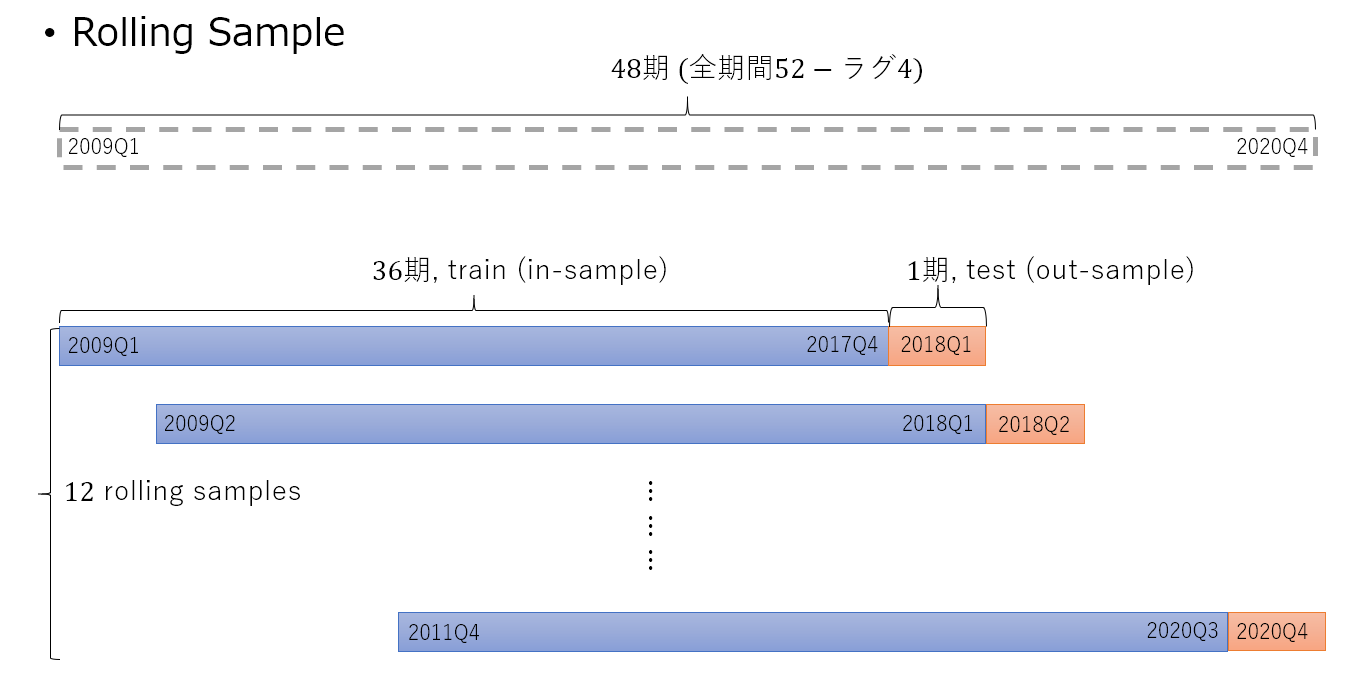
\includegraphics[width=12cm]{./img/_rolling_sample.png}
\end{figure}
% <!-- blender使って,企業の軸も入れて3Dにするとかっこいい? -->

\section{伝統的時系列モデル}

\subsection{ランダムウォーク}

$Y_t$をある企業におけるt期の四半期EPSとすると,もっとも単純な単変量モデルであるランダムウォークは次のとおりである.

\begin{equation}
  \begin{split}
    & Y_t = Y_{t-1} + \epsilon_t \\
    & \hat{Y}_t^{RW} = Y_{t-1} \\
  \end{split}
\end{equation}        

%     \\
%     & ただし,\epsilon_t は全ての時点 t において \\
%     & E[\epsilon_t] = 0 \\
%     & E[\epsilon_t \epsilon_{t-k}] = \left\{
%         \begin{array}{ll}
%         \sigma^2 & k=0 \\
%         0 & k \neq 0
% \end{array}\right.\\
%     & を満たすホワイトノイズである.\\
%     \\

ただし,$\epsilon_t$は全ての時点tにおいて
\begin{equation}
  \begin{split}
    & E[\epsilon_t] = 0 \\
    & E[\epsilon_t \epsilon_{t-k}] = \left\{
      \begin{array}{ll}
        \sigma^2 & k=0 \\
        0 & k \neq 0
      \end{array}\right.\\
  \end{split}
\end{equation}    

を満たすホワイトノイズである.

一方,四半期EPS時系列には1年単位での季節的変動パターンがあると考えられる.そこでランダムウォーク過程を1四半期単位ではなく,1会計年度単位(4四半期)であると考慮した季節ランダムウォークが次のとおりである.

\begin{equation}
  \begin{split}
    & Y_t = Y_{t-4} + \epsilon_t \\
    & \hat{Y}_t^{SRW} = Y_{t-4} \\
  \end{split}
\end{equation} 

ランダムウォークは前四半期の実績値を,季節ランダムウォークは前年同四半期の実績値を予測値とするモデルであり,どちらも実際の予測においてパラメータを推定する工程がない単純なモデルである.そこで,本稿ではランダムウォーク及び季節ランダムウォークを他の予測に対するベンチマークとして用いる.

\subsection{ARIMAモデル}

従来の四半期EPSを予測する単変量線形時系列モデルとして,自己回帰和分移動平均(AutoRegressive Integrated Moving Average: ARIMA)モデル\citep{box2015time}\footnote{ARIMAモデルは提唱者の名前からBox-Jenkinsモデルとも呼ばれる.},特にデータの季節性にも対応できるように一般化した季節自己回帰和分移動平均(Seasonal AutoRegressive Integrated Moving Average: SARIMA)モデルを用いる.$B^nY_t = y_{t-n}$ と定義されるような$B$(backshift operator)を導入すると,SARIMAモデルの一般形は以下のとおりである.\footnote{定数項$\theta_{\mu}=(1-\phi_1-\cdots-\phi_p)\mu$は階差をとれば0となるため,通常の取り扱いに従って0とする.}

\begin{equation}
  \begin{split}
    \phi_p(B)\Phi_{P}(B)(1-B)^d(1-B^s)^DY_t &= \theta_q(B)\Theta_Q(B^s)\epsilon_t
  \end{split}
\end{equation}

ただし,
\begin{equation}
  \begin{split}
    p &: トレンドの自己回帰過程の階数 \\
    d &: トレンド階差の次数 \\
    q &: トレンドの移動平均過程の階数 \\
    P &: 季節変動の自己回帰過程の階数 \\
    D &: 季節階差の次数 \\
    Q &: 季節変動の移動平均過程の階数 \\
    s &: 季節変動の周期 \\
    \phi_p(B) &= (1 - \phi_1B - \cdots - \phi_pB^p) \\
    \theta_q(B) &= (1 - \theta_1B - \cdots - \theta_qB^q) \\
    \Phi_P(B^s) &= (1 - \Phi_1B^s - \cdots - \Phi_PB^{sP}) \\
    \Theta_Q(B^s) &= (1 - \Theta_1B^s - \cdots - \Theta_QB^{sQ}) \\
  \end{split}
\end{equation}

通常,SARIMAモデルは$(p,d,q) \times (P,D,Q)$の値の組み合わせをBox-Jenkins法によってデータごとに選定し,モデルの構築を行う.一方,これまでの四半期EPSの時系列予測の分野では全ての企業に適合するSARIMAモデルが探求され,次の3つのSARIMAモデル\citep*{foster1977quarterly, griffin1977time, brown1979univariate}があらゆる企業の四半期EPSの時系列特性を描写するモデルであるとされている.
% \footnote{先行研究では,企業ごとにモデルを構築するよりも,企業で共通の構築で予測したほうが全体として予測のパフォーマンスが良いと示されている.}

\cite{foster1977quarterly} $: (p,d,q) \times (P,D,Q)_s = (1,0,0) \times (0,1,0)_4$

\begin{equation}
  \begin{split}
    % \text{ Foster (1977) } &: (p,d,q) \times (P,D,Q)_s = (1,0,0) \times (0,1,0)_4 \\
    Y_t &= Y_{t-4} + \phi_1(Y_{t-1} - Y_{t-5}) + \epsilon_t \\
    \hat{Y}_t^{ARIMA-F} &= Y_{t-4} + \phi_1(Y_{t-1} - Y_{t-5}) + \delta \\
  \end{split}
\end{equation}

\cite{griffin1977time} $: (p,d,q) \times (P,D,Q)_s = (0,1,1) \times (0,1,1)_4$

\begin{equation}
  \begin{split}
    Y_t &= Y_{t-4} + (Y_{t-1} - Y_{t-5}) - \theta_1a_{t-1} - \Theta_1a_{t-4} + \theta_1\Theta_1a_{t-5} + \epsilon_t \\
    \hat{Y}_t^{ARIMA-G} &= Y_{t-4} + (Y_{t-1} - Y_{t-5}) - \theta_1a_{t-1} - \Theta_1a_{t-4} + \theta_1\Theta_1a_{t-5} + \delta \\
  \end{split}
\end{equation}

\cite*{brown1979univariate} $: (p,d,q) \times (P,D,Q)_s = (1,0,0) \times (0,1,1)_4$

\begin{equation}
  \begin{split}    
    Y_t &= Y_{t-4} + \phi_1(Y_{t-1}-Y_{t-5}) - \Theta_1a_{t-4} + \epsilon_t \\
    \hat{Y}_t^{ARIMA-BR} &= Y_{t-4} + \phi_1(Y_{t-1}-Y_{t-5}) - \Theta_1a_{t-4} + \delta \\
    \\
  \end{split}
\end{equation}

ただし,$\delta$はSARIMAモデルの定数項である.

本稿では先行研究に倣い,特に支持されてきたこの3つのモデルを単変量線形時系列モデルとして用いることとする.

\subsection{多変量線形モデル}

ファンダメンタル会計変数が将来の四半期EPSを線形に説明するかどうかについて確かめるため,\cite*{lev1993fundamental},\cite*{abarbanell1997fundamental},\cite*{lorek1996multivariate}の研究で用いられているモデルをもとに,以下のような多変量線形回帰モデルを考える.

\begin{equation}
  \begin{split}
    \label{eq:ols1}
    \hat{Y}_t^{OLS1} = \beta_0 + \beta_1Y_{t-1} + \beta_2Y_{t-4} 
    &+ \beta_3INV_{t-1} + \beta_4AR_{t-1} + \beta_5CAPX_{t-1} \\
    &+ \beta_6GM_{t-1} + \beta_7SA_{t-1} + \beta_8ETR_{t-1} + \beta_9LF_{t-1} \\
  \end{split}
\end{equation}

\begin{equation}
  \begin{split}
    \label{eq:ols2}
    \hat{Y}_t^{OLS2} = \beta_0 + \beta_1Y_{t-1} + \beta_2Y_{t-4} 
    &+ \beta_3INV_{t-4} + \beta_4AR_{t-4} + \beta_5CAPX_{t-4} \\
    &+ \beta_6GM_{t-4} + \beta_7SA_{t-4} + \beta_8ETR_{t-4} + \beta_9LF_{t-4} \\
  \end{split}
\end{equation}

2つのモデルはどちらも,四半期EPSの1四半期前ラグ$Y_{t-1}$と4四半期前ラグ$Y_{t-4}$が自己回帰的な説明変数として含まれている.両者の違いとしてはファンダメンタル会計変数のラグの次数にあり,(\ref{eq:ols1})のモデルではファンダメンタル会計変数の1四半期前ラグを,(\ref{eq:ols2})のモデルでは季節性を考慮してファンダメンタル会計変数の4四半期前ラグをモデルの説明変数として含めている.一方,Cao and Parry (2009) は後述する機械学習アルゴリズムのモデルと利用できる情報の公平性に保つため,以下のように四半期EPSとファンダメンタル会計変数のラグ変数を1四半期前,2四半期前,3四半期前,4四半期前すべて含めた多変量線形回帰モデルを推定している.

\begin{equation}
  \begin{split}
    \label{eq:ols3}
    \hat{Y}_t^{OLS3} = \beta_0 + \sum^{4}_{\tau=1} \left( \beta_{1\tau}Y_{t-\tau} 
    + \beta_{2\tau}INV_{t-\tau} + \beta_{3\tau}AR_{t-\tau} + \beta_{4\tau}CAPX_{t-\tau} \right.\\
    \left.+ \beta_{5\tau}GM_{t-\tau} + \beta_{6\tau}SA_{t-\tau} + \beta_{7\tau}ETR_{t-\tau} + \beta_{8\tau}LF_{t-\tau} \right) \\
  \end{split}
\end{equation}

以上のファンダメンタル会計変数を説明変数として用いた3つの多変量線形回帰モデルを多変量モデルのベンチマークとして,他の手法による多変量予測と比較する.
% なお,これらのモデルのパラメータは最小二乗法を用いてを推定する.
% 推定法っていわなくてもいい?

\section{機械学習モデル}

% 金融データは高次元,7変数しかもラグ,普通のモデルは変数多いと精度下がる.機械学習で次元削減.
% 金融データは非線形.非線形なモデル2つ.AnnとノンパラなRF

ここでは,本稿で用いる機械学習的手法について紹介する.なお,以下より共通して時点$t$の説明変数ベクトル$\bm{X}_t$について,単変量モデルでは目的変数である四半期EPSのラグのみを用いてモデル構築を行う.

\begin{equation}
  \begin{split}
    \bm{X}_t &= (X_{t1},\cdots ,X_{tk}) \\
    &= (Y_{t-1},Y_{t-2},Y_{t-3},Y_{t-4}) \\
  \end{split}
\end{equation}

また,多変量モデルでは四半期EPSのラグに加え,ファンダメンタル会計変数のラグも含めてモデルを構築する.

\begin{equation}
  \begin{split}
    \bm{X}_t = (&X_{t1},\cdots ,X_{tk}) \\ 
    =(&Y_{t-1},Y_{t-2},Y_{t-3},Y_{t-4},\\
    & INV_{t-1},INV_{t-2},INV_{t-3},INV_{t-4},\\
    & AR_{t-1},AR_{t-2},AR_{t-3},AR_{t-4},\\
    & CAPX_{t-1},CAPX_{t-2},CAPX_{t-3},CAPX_{t-4},\\
    & GM_{t-1},GM_{t-2},GM_{t-3},GM_{t-4},\\
    & SA_{t-1},SA_{t-2},SA_{t-3},SA_{t-4},\\
    & ETR_{t-1},ETR_{t-2},ETR_{t-3},ETR_{t-4},\\ 
    & LF_{t-1},LF_{t-2},LF_{t-3},LF_{t-4}) \\
  \end{split}
\end{equation}

\subsection{罰則回帰モデル}

説明変数間に複数の強い相関が存在する場合,線形回帰モデルの最小二乗推定量の分散は大きくなる.そして高分散(high variance)により係数の推定値が極端な値をとると,訓練データ内での予測精度は高くても,テストデータにおける予測精度が低くなる恐れがある.このように予測モデルが訓練データの規則性のみを捉えてしまい,テストデータを含めたデータ全体に対して汎化できていないことを過学習(overfitting)という.

線形回帰モデルの係数の推定値が極端な値をとることに起因する過学習を防ぐために,係数の大きさに罰則を与えて推定する手法が罰則回帰モデル(penalized regression model)である\footnote{罰則回帰モデルの詳細については,\cite*{hoerl1970ridge, tibshirani1996regression, zou2005regularization}などを参照されたい.}.罰則回帰モデルは,その罰則の与え方によって推定で最小化する目的関数が異なる.本稿では罰則回帰モデルのうち,代表的なRidge回帰,LASSO回帰,Elastic Net回帰の3つを用いる.

Ridge回帰の係数は次のとおりである.

\begin{equation} \label{eq:ridge}
  \begin{split}
    \hat{\bm{\beta}}^{Ridge} = \argmin_{\bm{\beta}}\left\{ \sum_{t=1}^{T} \left( Y_t - \beta_0 - \sum_{j=1}^{k} \beta_{j} X_{tj} \right)^2 + \lambda \sum_{j=1}^{k} \beta_{j}^{2} \right\}
  \end{split}
\end{equation}

ここで,$\lambda \geq 0$は罰則の強さを調節するパラメータであり,モデル推定の枠組みの中で決定されないパラメータ(ハイパーパラメータ)である.ハイパーパラメータの値はデータに応じて指定する必要があり,本稿におけるハイパーパラメータの選択方法の詳細については\ref{sec:hyparam}節で説明する.(\ref{eq:ridge})式で示されるように,Ridge回帰では目的関数に係数の二乗和が含まれており,係数が過大な値をとることを防ぐ構造となっている.したがってRidge回帰は予測情報を持たない説明変数に対して係数縮小(parameter shrinkage)し,モデルの過学習を防ぐ.

LASSO(Least Absolute Shrinkage and Selection Operator)回帰モデルの係数は次のとおりである.

\begin{equation} \label{eq:lasso}
  \begin{split}
    \hat{\bm{\beta}}^{LASSO} = \argmin_{\bm{\beta}}\left\{ \sum_{t=1}^{T} \left( Y_t - \beta_0 - \sum_{j=1}^{k} \beta_{j} X_{tj} \right)^2 + \lambda \sum_{j=1}^{k} \left|\beta_{j}\right| \right\}
  \end{split}
\end{equation}

LASSO回帰は,Ridge回帰と同様,目的関数にパラメータのサイズに関する罰則項が含まれているが,罰則として係数の絶対値の和を用いている点がRidge回帰との違いである.この罰則の与え方により,予測情報を持たない説明変数の係数が丁度0となるスパース推定が行われる.つまり,LASSO回帰を推定することで変数選択が行われる.

Elastic Net回帰の係数は次のとおりである.

\begin{equation}
  \begin{split}
    \hat{\bm{\beta}}^{EN} = \argmin_{\bm{\beta}}\left\{ \sum_{t=1}^{T} \left( Y_t - \beta_0 - \sum_{j=1}^{k} \beta_{j} X_{tj} \right)^2 + 
    \lambda \left\{ 
      \left( 1 - \alpha \right) \sum_{j=1}^{k} \beta_{j}^2 + 
      \alpha \sum_{j=1}^{k} \left|\beta_{j}\right| 
      \right\} 
    \right\}
  \end{split}
\end{equation}

Elastic Net回帰は,Ridge回帰とLASSO回帰両方の罰則項を利用する構造となっている.$\alpha$はLASSO回帰の罰則の影響の割合を調節するハイパーパラメータであり,罰則の強さを調節するハイパーパラメータ$\lambda$と併せて指定する必要がある.

なお,それぞれの罰則回帰モデルの予測値は次のとおりである.

\begin{equation}
  \begin{split}
    \hat{Y}_t^{Ridge} &= \beta_0^{Ridge} + \sum_{j=1}^{k} \beta_{j}^{Ridge} X_{tj} \\
    \hat{Y}_t^{LASSO} &= \beta_0^{LASSO} + \sum_{j=1}^{k} \beta_{j}^{LASSO} X_{tj} \\
    \hat{Y}_t^{EN} &= \beta_0^{EN} + \sum_{j=1}^{k} \beta_{j}^{EN} X_{tj} \\
  \end{split}
\end{equation}

\subsection{ランダムフォレスト回帰}

ランダムフォレスト\citep{breiman2001random}は,決定木を弱学習器とするアンサンブル学習である.弱学習器とはそれ単独で用いると精度が低いような予測モデルであり,アンサンブル学習はその弱学習器を複数推定し,組み合わせることで予測精度の向上を図る手法である.弱学習器となる決定木は,ある変数のある閾値でデータを2分割し,この分割を繰り返すことで作成される.単独の決定木による予測値は,予測サンプルの説明変数をもとに作成された木の分岐を辿り,到達した末端ノードに属するサンプルの目的変数の平均値である.ランダムフォレスト回帰では,元のデータセットから標本及び変数を無作為に復元抽出した複数のサブデータセットを構築し(ブートストラップサンプリング),それをもとに弱学習器である決定木を複数推定する.そして各決定木の予測値の平均値が最終的なランダムフォレスト回帰の予測値となる.

% ランダムフォレストのイラスト?https://www.stats-guild.com/analytics/12543

決定木の数を$M$とし,$m=1,\cdots M$番目の決定木の$t$時点における予測値を$\textit{Tree}_m(\bm{X}_t)$とすると,ランダムフォレスト回帰の予測値は以下のように表される.

\begin{equation}
  \begin{split}
    \hat{Y}_t^{RF} = \frac{1}{M} \sum_{m=1}^{M} \textit{Tree}_m(\bm{X}_t)
  \end{split}
\end{equation}

なお,ランダムフォレスト回帰の複雑さを調節する決定木の数や決定木の分岐の回数(木の深さ)はハイパーパラメータであり,分析者が指定する必要がある.

ランダムフォレスト回帰は,ノンパラメトリックで非線形なモデルであり,説明変数と目的変数間に非線形な関係がある場合でも優れた予測が得られると考えられる.また,ブートストラップをもとに相関のない複数の決定木を推定して各決定木の予測値の平均を用いて予測を行うため,最終的な予測値の分散は小さく,予測の汎化性能が高まる性質を持つ.

\subsection{ニューラルネットワークモデル}

ニューラルネットワーク(Neural Network: NN)について述べる.まずNNの構造の最小単位であるパーセプトロンについて考える.$\bm{X_t}=(X_{t1},\cdots,X_{tk})$を入力(説明変数)ベクトルとする.$(w_1,\cdots,w_k)$は入力ベクトルの要素それぞれに対応する重み(パラメータ)であり,スカラー値$b$はバイアス項(定数項)という.パーセプトロンではまず始めに$\bm{X_t}=(X_{t1},\cdots,X_{tk})$と$(w_1,\cdots,w_k)$の内積と$b$の和であるプレアクティベーション$z$を計算する.

\begin{equation}
  \begin{split}
    z = w_1 X_{t1} + \cdots + w_k X_{tk} + b
  \end{split}
\end{equation}

次に$z$は非線形な関数である活性化関数 $\phi(\cdot)$ に渡され,アクティベーション$a$として出力される.

\begin{equation}
  \begin{split}
    a = \phi(z)
  \end{split}
\end{equation}

以上がNNのパーセプトロンの構造であり,まとめると以下の式で表される.

\begin{equation}
  \begin{split}
    a = \phi \left(w_1 X_{t1} + \cdots + w_k X_{tk} + b \right)
  \end{split}
\end{equation}

このパーセプトロンを複数組み合わせることで,NNが構成される.

NNと一口に言ってもその構造によって様々な種類のものがある.NNの1種である順伝播型ニューラルネットワーク(Feed-forward Neural Network: FNN)はNNのなかでも基本的な構造を持ち,全てのパーセプトロンが結合した無閉路グラフで表現されすべての計算が逐次的に行われる.FNNの最も代表的なネットワークは多層パーセプトロン(multilayer perceptron: MLP)であり,図\ref{fig:perceptron}のように表される.

\begin{figure}
  \centering
  \caption{パーセプトロンのイメージ}
  \label{fig:perceptron}
  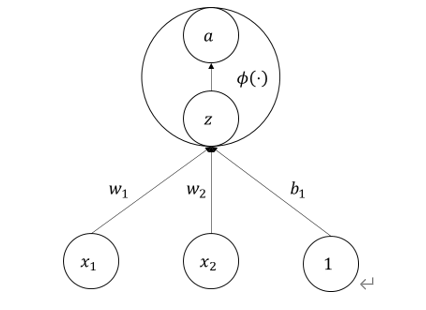
\includegraphics[width=7cm]{./img/_ann_unit.png}
\end{figure}

MLPの特徴として,横のつながりのパーセプトロンをそれぞれ層としてまとめると少なくとも3つ以上の層から構成される.またMLPはネットワークの全てのパーセプトロンが次の層に含まれる全てのパーセプトロンとそれぞれ結合している.ネットワークの最初の層は入力層といい入力される特徴量がここにあたる.最後の層は出力層といい,ネットワークが出力する値であり,出力層のアクティベーションは予測値を表す.この2つを除いた間の層は全て隠れ層といい,MLPの多層構造を作る.

例えば,入力層と1層の隠れ層,出力層から成る3層パーセプトロンを定式化してみる.まず,隠れ層のアクティベーションをベクトル$(H_{t1},\cdots,H_{tL})$とする.ただし,$L$は隠れ層に含まれるパーセプトロンの数である.また,隠れ層の活性関数を $\phi^{(1)}(\cdot)$ とし,隠れ層のバイアス項を$(b^{(1)}_1,\cdots,b^{(1)}_L)$とすると,隠れ層のアクティベーションは以下のように表される.

\begin{equation}
  \begin{split}
    H_{t1} &= \phi^{(1)} \left( w^{(1)}_{11} X_{t1} + w^{(1)}_{21} X_{t2} + \cdots + w^{(1)}_{k1} X_{tk} + b^{(1)}_1 \right) \\
    H_{t2} &= \phi^{(1)} \left( w^{(1)}_{12} X_{t1} + w^{(1)}_{22} X_{t2} + \cdots + w^{(1)}_{k2} X_{tk} + b^{(1)}_2 \right) \\
    \vdots \\
    H_{tL} &= \phi^{(1)} \left( w^{(1)}_{1L} X_{t1} + w^{(1)}_{2L} X_{t2} + \cdots + w^{(1)}_{kL} X_{tk} + b^{(1)}_L \right) \\
  \end{split}
\end{equation}

 次に,出力層について考える.予測する変数は本稿では1次元であるため,出力層のアクティベーションはスカラー$Y$となる.出力層の活性関数を$\phi^{(2)}(\cdot)$とし,バイアス項を$b^{(2)}$とすると,出力層のアクティベーション(または予測値)は以下のように表される.図\ref{fig:mlp}はMLPのイメージを表している.

\begin{equation}
  \begin{split}
    \hat{Y}_t = \phi^{(2)} \left( w^{(2)}_{1} H_{t1} + w^{(2)}_{2} H_{t2} + \cdots + w^{(2)}_{L} H_{tL} + b^{(2)} \right)
  \end{split}
\end{equation}

\begin{figure}
  \centering
  \caption{MLPのイメージ}
  \label{fig:mlp}
  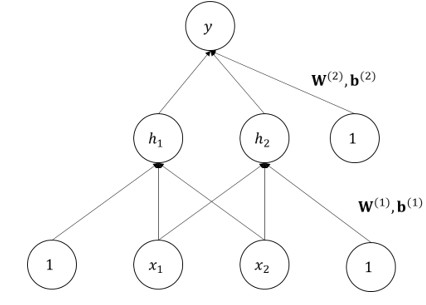
\includegraphics[width=7cm]{./img/_ann_mlp.png}
\end{figure}

このように,MLPは線形結合モデルを非線形変換したものの繰り返しであることがわかる.このMLPの隠れ層の数を増やすことで,ネットワークをより深くすることができ,深層ニューラルネットワークが構築できる.一方,\cite{qi1999nonlinear}は,隠れ層のパーセプトロン数が十分であれば,隠れ層が1つで,隠れ層の活性化関数にロジスティック関数,出力層の活性化関数に恒等関数を用いた3層パーセプトロンは,あらゆる連続関数を近似できると述べている.そこで本稿は,\cite{callen1996neural}や\cite{zhang2004neural}と同様に以下のような3層パーセプトロンを用いる.

\begin{equation}
  \begin{split}
    \hat{Y}_t^{NN} 
    &= f({\bm{X}_t,\alpha,\beta}) \\
    &= \sum^{L}_{l=1} \left(\alpha_0 + \alpha_l H_{tl} \right) \\
    &= \sum^{L}_{l=1} \left\{ \alpha_0 + \alpha_l \textit{logistic} \left(\sum^{k}_{j=1} \left(\beta_{0l} + \beta_{jl} X_{tj} \right) \right) \right\} \\
  \end{split}
\end{equation}

ただし,

\begin{equation}
  \begin{split}
    \bm{X}_t &: 時点tの入力ベクトル \\
    X_{tk} &: k番目の入力 \\
    L &: 隠れ層のパーセプトロン数 \\
    \alpha_l &: 隠れ層のl番目のパーセプトロンと目的変数の重み \\
    \alpha_0 &: 出力層のバイアス項 \\
    \beta_{jl} &: j番目の入力とl番目の隠れ層のパーセプトロンの重み \\
    \beta_{0l} &: 隠れ層のl番目のパーセプトロンのバイアス項 \\
    \textit{logistic}(\cdot) = \frac{\exp(\cdot)}{1 + \exp(\cdot)} &: ロジスティック関数
  \end{split}
\end{equation}

NNの推定は誤差逆伝播法(Backward propagation algorithm)を用いて重みの勾配を計算し,勾配降下によって行う.なお,NNの複雑さを調節する隠れ層のパーセプトロン数と,重みの更新量の幅を調節する学習率はハイパーパラメータであり,分析者が指定する必要がある.

\section{ハイパーパラメータの選択} \label{sec:hyparam}

多くの機械学習アルゴリズムには,モデル推定の枠組みでは決定されない,分析者が指定する必要のあるハイパーパラメータが存在する.ハイパーパラメータの値が正しく設定できていないと,それをもとに推定されたモデルは過学習もしくは学習不足\footnote{過学習の反対語で,訓練データの規則性を十分とらえきれていないことを意味する.例えば,罰則付き回帰の罰則の強さを表す$\lambda$の値がデータに対して大きすぎる場合,係数の大きさに対する罰則が必要以上に強く,モデルがデータの規則性を十分に学習できない可能性が生じる.}となる恐れがあり,未知のデータに対して汎化性能を持たず,高い予測精度が期待できない.そこで本稿では適切なハイパーパラメータの値を設定するため,企業ごとにグリッドサーチを行う.

具体的には,ある1企業の12個のローリングサンプルそれぞれの訓練データのうち,最新時点のデータをあらたに検証データ(validation data)として分割する.例えば1つ目のローリングサンプル$\left\{Data_{\text{2008Q1}}, Data_{\text{2008Q2}}, \cdots, Data_{\text{2017Q3}}, Data_{\text{2017Q4}}, Data_{\text{2018Q1}}\right\}$では,訓練データを$\left\{Data_{\text{2008Q1}}, Data_{\text{2008Q2}}, \cdots, Data_{\text{2017Q3}}\right\}$,検証データを$\left\{Data_{\text{2017Q4}}\right\}$,テストデータを$\left\{Data_{\text{2018Q1}}\right\}$として3つに分割する.この分割を12個のローリングサンプルに対して行い,12個の検証データ$\left\{Data_{\text{2017Q4}}, \cdots , Data_{2020Q3}\right\}$を得る.次に,候補となるハイパーパラメータの組を用意し,全通りのハイパーパラメータをそれぞれ用いて,訓練データのみをもとに12個のモデルを推定し,検証データの目的変数を予測する.そして,検証データに対する予測能力が最も高いハイパーパラメータの組合せを最適なモデル設定であるとする.最終的には,最適なハイパーパラメータをもとに訓練データと検証データの両方を用いてモデルを再推定し,テストデータの目的変数を予測する.図\ref{fig:hyparam_selection}は本稿におけるハイパーパラメータ選択のイメージを表している.

% なお,本稿で用いた各機械学習モデルのハイパーパラメータの候補はAppendixに記載している.

\begin{figure}
  \centering
  \caption{ハイパーパラメータ選択のイメージ}
  \label{fig:hyparam_selection}
  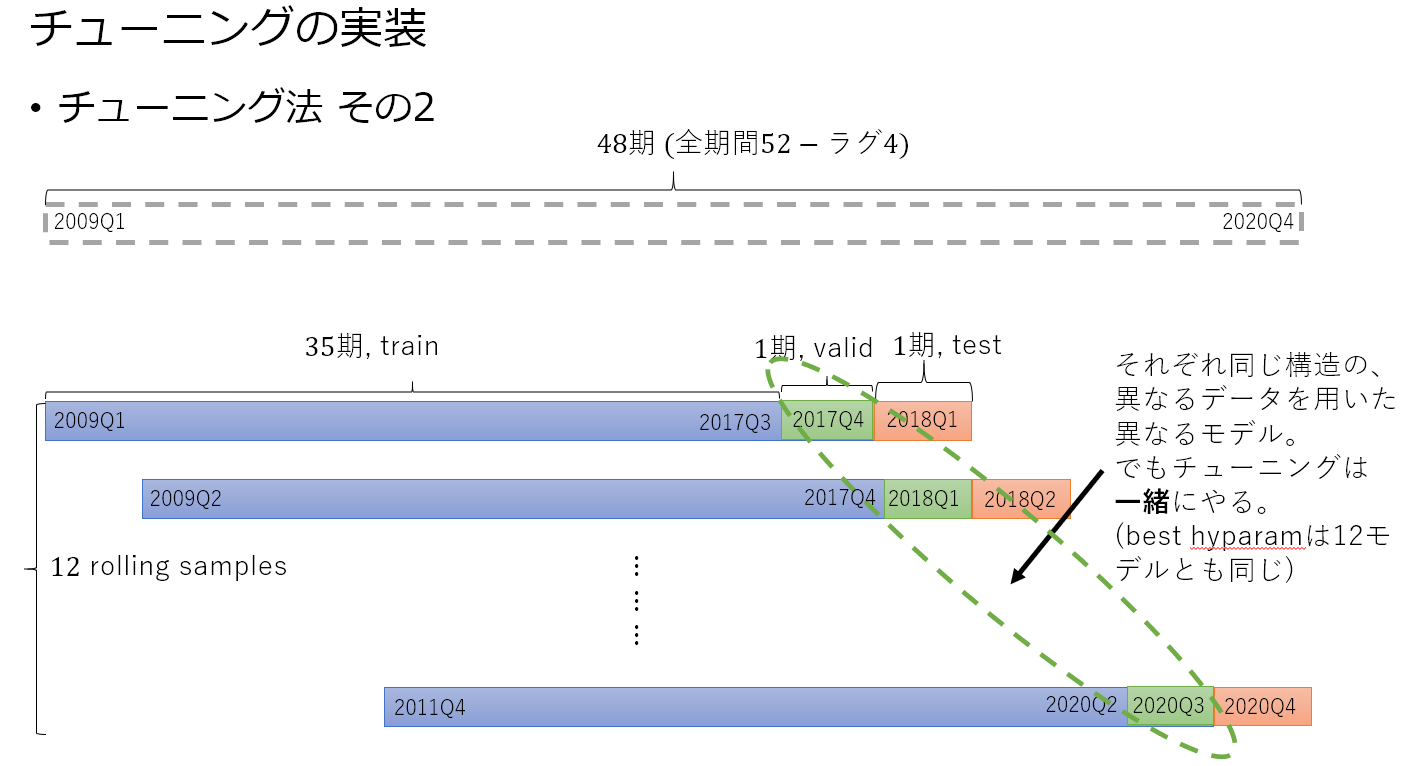
\includegraphics[width=12cm]{./img/_rolling_sample_val_i.png}
\end{figure}

% \part{予測精度の比較方法}

\section{予測精度指標}

各モデルの四半期EPS予測の精度を測るために,以下の予測精度指標を用いる.

平均絶対誤差(Mean Absolute Error: MAE)

\begin{equation}
  \begin{split}
    \text{MAE} = \frac {1} {T} \sum^{T}_{t=1}\left| Y_t - \hat{Y}_t \right|
  \end{split}
\end{equation}

平均絶対誤差率(Mean Absolute Percentage Error: MAPE)

\begin{equation}
  \begin{split}
    \text{MAPE} = \frac {1} {T} \sum^{T}_{t=1}\left| \frac {Y_t - \hat{Y}_t} {Y_t} \right|
  \end{split}
\end{equation}

平均二乗誤差率(Mean Squared Percentage Error: MSPE)

\begin{equation}
  \begin{split}
    \text{MSPE} = \frac {1} {T} \sum^{T}_{i=1} \left( \frac {Y_t - \hat{Y}_t} {Y_t} \right) ^2
  \end{split}
\end{equation}

ただし,$T$は予測期間であり,本稿では2018年度第1四半期~2020年度第4四半期の12期間である.なお,絶対予測誤差率$ \left| \frac{Y_t -{\hat Y}_t}{Y_t} \right|$が1を超える予測サンプルについては,\cite*{brown1979univariate},\cite*{lorek1996multivariate},\cite{zhang2004neural}に倣い絶対予測誤差率の上界を1とし,この制約に基づいて算出した精度指標を報告することとする.また,そのような予測サンプルはLarge Forecast Errorサンプルとし,予測精度指標の値と併せてLarge Forecast Errorの割合も報告する.

\section{Diebold-Mariano(DM)検定}

予測精度指標は異なる予測モデル間で予測精度を比較するために用いられる.一方,精度指標の値は本稿で用いているデータセットのみに由来しているため,精度指標の大小関係を比較するだけではモデルの精度の優劣を一般化することはできない.そこで,本稿では異なる2つの予測モデル間に統計的に有意な予測精度の差が存在するかどうかを検定するために,Diebold-Mariano(DM)検定\citep*{diebold2002comparing}を行う.

具体的には,ある企業について,予測期間の実績値(真の値)を$\left\{Y_t; t=1, \cdots, T\right\}$,異なる2つの予測モデル(モデル1とモデル2)に由来する予測値系列をそれぞれ$\left\{\hat{Y}_{1t}; t=1, \cdots, T\right\}, \left\{\hat{Y}_{2t}; t=1, \cdots, T\right\}$とする.このとき予測誤差系列をそれぞれ,

\begin{equation}
  \begin{split}
    \left\{ e_{1t} = \hat{Y}_{1t} - Y_t ; t=1, \cdots, T \right\} \\
    \left\{ e_{2t} = \hat{Y}_{2t} - Y_t ; t=1, \cdots, T \right\} \\
  \end{split}
\end{equation}

\noindent
とし,予測誤差の損失$L(e_t)$\footnote{損失関数$L(e_t)$は用いる予測精度指標によって異なる.例えば,MAEの場合は$L(e_t)=|e_t|$,MAPEの場合は$L(e_t)=\left|\frac{e_t}{Y_t}\right|$,MSPEの場合は$L(e_t)=\left(\frac{e_t}{Y_t}\right)^2$となる.}をもとに2つの予測誤差系列の損失差$d_{12t}$を以下のように定義する.

\begin{equation}
  \begin{split}
    d_{12t} = L(e_{1t}) - L(e_{2t})
  \end{split}
\end{equation}

モデル1とモデル2の予測誤差に差がないとき,損失差の期待値は0となる.つまり,DM検定の帰無仮説と対立仮説は次のとおりである.

\begin{equation}
  \begin{split}
    H_0 &: E(d_{12t}) = 0,  \\
    H_1 &: E(d_{12t}) \neq 0
  \end{split}
\end{equation}

この仮説検定を行うために以下のような検定統計量,

\begin{equation}
  \begin{split}
    DM_{12} &= \frac {\bar{d}_{12}} {s.e.(\bar{d}_{12})} \\
    &ただし,\\
    &\bar{d}_{12} = \frac {1} {T} \sum^{T}_{t=1} d_{12t} \\
    &s.e.(\bar{d}_{12}) は\bar{d}_{12}の標準誤差.\\
  \end{split}
\end{equation}

\noindent
を導入し,$d_{12t}$について緩い仮定の下で$DM_{12}$が標準正規分布に漸近的分布することを用いる\footnote{DM検定の詳細については\cite{diebold2002comparing}を参照されたい.}.両側DM検定で統計的に有意な検定結果が得られなければ,モデル1とモデル2の間に予測パフォーマンスの統計的有意な差がない結果となる.DM検定量が正の値で統計的に有意であれば,モデル1の予測誤差はモデル2よりも大きく,モデル2の方が優れた予測を与えるという結果となる.反対に,DM検定量が負の値で統計的に有意であれば,モデル1の予測誤差はモデル2よりも小さく,モデル1の方が優れた予測を与えるという結果となる.

\part{予測結果} \label{par:result}

\section{時系列モデル間の予測精度比較}

% T=4, T=4. T=4, T=12 行の挿入
\begin{landscape}
\begin{table}
  % \centering
  \caption{時系列モデルによる1期先四半期EPS予測の精度(1,003社平均)}
  \label{tab:acc}
  \scalebox{0.75}[0.75]{
    %%% threeparttable %%%
\begin{threeparttable}[h]

% \begin{tabular}{lrrrrrrrrrrrrrrrrrrrr}
\begin{tabular}{lrrrp{1.5cm}rrrp{1.5cm}rrrp{1.5cm}rrrp{1.5cm}rrrp{1.5cm}}
% \begin{tabularx}{6cm}{lrrrXrrrXrrrXrrrXrrrX}

\toprule
{} & \multicolumn{4}{c}{Q1} & \multicolumn{4}{c}{Q2} & \multicolumn{4}{c}{Q3} & \multicolumn{4}{c}{Q4} & \multicolumn{4}{c}{Overall} \\
\cmidrule(lr){2-5}
\cmidrule(lr){6-9}
\cmidrule(lr){10-13}
\cmidrule(lr){14-17}
\cmidrule(lr){18-21}
% \tnote
{} &    MAE \tnote{b}&   MAPE \tnote{c}&   MSPE \tnote{d}& Large Forecast Error(\%) \tnote{e}&    MAE &   MAPE &   MSPE & Large Forecast Error(\%) &    MAE &   MAPE &   MSPE & Large Forecast Error(\%) &    MAE &   MAPE &   MSPE & Large Forecast Error(\%) &     MAE &   MAPE &   MSPE & Large Forecast Error(\%) \\
% \tnote
Model \tnote{a}     &        &        &        &                         &        &        &        &                         &        &        &        &                         &        &        &        &                         &         &        &        &                         \\
\midrule
U-RW       &   44.2 &  0.668 &  0.572 &                    42.6 &   27.6 &  0.529 &  0.408 &                    25.7 &   29.7 &  0.499 &  0.372 &                    22.3 &   47.9 &  0.621 &  0.514 &                    36.1 &    37.3 &  0.579 &  0.467 &                    31.7 \\
U-SRW      &   27.1 &  0.547 &  0.436 &                    27.8 &   27.4 &  0.505 &  0.390 &                    23.8 &   26.3 &  0.461 &  0.338 &                    20.4 &   47.2 &  0.573 &  0.464 &                    32.2 &    32.0 &  0.521 &  0.407 &                    26.0 \\
U-ARIMA-F  &   32.6 &  0.549 &  0.437 &                    29.5 &   25.7 &  0.480 &  0.362 &                    22.4 &   28.3 &  0.477 &  0.355 &                    21.4 &   46.7 &  0.573 &  0.463 &                    32.3 &    33.3 &  0.520 &  0.404 &                    26.4 \\
U-ARIMA-G  &   37.7 &  0.567 &  0.460 &                    32.4 &   30.9 &  0.481 &  0.366 &                    23.9 &   33.2 &  0.488 &  0.370 &                    23.5 &   50.2 &  0.570 &  0.461 &                    31.8 &    38.0 &  0.526 &  0.414 &                    27.9 \\
U-ARIMA-BR &   36.4 &  0.559 &  0.445 &                    29.3 &   29.2 &  0.482 &  0.362 &                    22.5 &   30.1 &  0.471 &  0.348 &                    21.0 &   47.7 &  0.564 &  0.452 &                    30.1 &    35.8 &  0.519 &  0.402 &                    25.7 \\
M-OLS1     &   64.1 &  0.626 &  0.527 &                    38.8 &   50.6 &  0.556 &  0.447 &                    32.0 &   40.4 &  0.528 &  0.414 &                    27.4 &   60.9 &  0.603 &  0.499 &                    35.4 &    54.0 &  0.578 &  0.472 &                    33.4 \\
M-OLS2     &   62.5 &  0.613 &  0.514 &                    38.0 &   44.0 &  0.549 &  0.439 &                    30.8 &   77.5 &  0.569 &  0.461 &                    32.4 &   84.4 &  0.625 &  0.526 &                    38.6 &    67.1 &  0.589 &  0.485 &                    35.0 \\
M-OLS3     &  333.8 &  0.821 &  0.769 &                    67.9 &  278.6 &  0.798 &  0.738 &                    63.8 &  263.9 &  0.790 &  0.727 &                    62.0 &  225.4 &  0.797 &  0.733 &                    62.7 &   275.4 &  0.801 &  0.742 &                    64.1 \\
U-RIDGE    &   41.9 &  0.576 &  0.469 &                    33.5 &   35.4 &  0.506 &  0.391 &                    26.2 &   37.0 &  0.499 &  0.373 &                    22.2 &   49.7 &  0.575 &  0.464 &                    31.5 &    41.0 &  0.539 &  0.424 &                    28.3 \\
U-LASSO    &   35.2 &  0.591 &  0.474 &                    28.9 &   31.0 &  0.530 &  0.401 &                    21.6 &   33.9 &  0.521 &  0.385 &                    18.4 &   45.5 &  0.592 &  0.473 &                    27.9 &    36.4 &  0.559 &  0.433 &                    24.2 \\
U-EN       &   34.0 &  0.581 &  0.462 &                    28.4 &   30.7 &  0.519 &  0.390 &                    21.4 &   32.7 &  0.510 &  0.372 &                    17.7 &   45.6 &  0.591 &  0.471 &                    27.6 &    35.7 &  0.550 &  0.423 &                    23.8 \\
U-RF       &   27.1 &  0.548 &  0.435 &                    28.8 &   25.0 &  0.480 &  0.358 &                    22.2 &   26.6 &  0.464 &  0.338 &                    19.2 &   40.8 &  0.561 &  0.445 &                    29.1 &    29.9 &  0.513 &  0.394 &                    24.8 \\
U-NN       &   50.7 &  0.624 &  0.515 &                    34.4 &   49.4 &  0.580 &  0.460 &                    28.2 &   49.4 &  0.554 &  0.430 &                    25.7 &   60.5 &  0.626 &  0.516 &                    34.0 &    52.5 &  0.596 &  0.480 &                    30.6 \\
M-RIDGE    &   38.1 &  0.527 &  0.419 &                    29.3 &   33.9 &  0.483 &  0.374 &                    25.1 &   36.6 &  0.468 &  0.355 &                    24.2 &   45.7 &  0.534 &  0.429 &                    30.3 &    38.6 &  0.503 &  0.394 &                    27.2 \\
M-LASSO    &   23.6 &  0.490 &  0.374 &                    23.1 &   23.5 &  0.438 &  0.321 &                    19.1 &   24.3 &  0.422 &  0.302 &                    17.2 &   38.1 &  0.495 &  0.382 &                    24.4 &    27.4 &  0.461 &  0.345 &                    21.0 \\
M-EN       &   22.9 &  0.479 &  0.362 &                    21.8 &   22.7 &  0.425 &  0.308 &                    18.2 &   23.7 &  0.417 &  0.296 &                    16.8 &   37.7 &  0.492 &  0.377 &                    23.7 &    26.8 &  0.453 &  0.336 &                    20.1 \\
M-RF       &   24.7 &  0.495 &  0.382 &                    25.7 &   21.2 &  0.413 &  0.295 &                    17.9 &   22.7 &  0.408 &  0.287 &                    17.2 &   36.8 &  0.513 &  0.398 &                    25.8 &    26.3 &  0.457 &  0.340 &                    21.7 \\
M-NN       &   35.8 &  0.588 &  0.480 &                    33.7 &   36.8 &  0.534 &  0.416 &                    27.1 &   33.0 &  0.517 &  0.392 &                    23.4 &   46.4 &  0.595 &  0.485 &                    33.4 &    38.0 &  0.558 &  0.443 &                    29.4 \\
\bottomrule
\end{tabular}

%%% table footnote %%%
\begin{tablenotes}
\item[a] 各モデルの先頭文字列U-は単変量モデル, M-は多変量モデルを表す. また, RWはランダムウオークモデル, SRWは季節ランダムウオークモデル, ARIMA-F, ARIMA-G, ARIMA-BRはそれぞれ\cite*{foster1977quarterly, griffin1977time, brown1979univariate}の設定のARIMAモデル, OLS1, OLS2, OLS3はそれぞれ式(\ref{eq:ols1}), 式(\ref{eq:ols2}), 式(\ref{eq:ols3})の線形回帰モデル, RIDGEはRidge回帰モデル, LASSOはLASSO回帰モデル, ENはElastic Net回帰モデル, RFはランダムフォレスト回帰モデル, NNはニューラルネットワークモデルを表す.
\item[b] 平均絶対誤差(Mean Absolute Error: MAE)
\item[c] 平均絶対誤差率(Mean Absolute Percentage Error: MAPE)
\item[d] 平均二乗誤差率(Mean Squared Percentage Error: MSPE)
\item[e] 絶対予測誤差率$\left| \frac{Y_t -{\hat Y}_t}{Y_t} \right|$が1を超えるLarge Forecast Errorサンプルについては絶対予測誤差率を1としており, 表に全予測サンプルに占めるLarge Forecast Errorサンプルの割合(\%)を示している.
\end{tablenotes}
\end{threeparttable}  
  }
\end{table}
\end{landscape}

表\ref{tab:acc}は各予測指標の全企業平均を四半期別と全予測期間で集計したものを示している.まず,単変量モデル間での予測精度を比較すると,全予測期間平均でMAE,MAPE,MSPEが最も小さいモデルはランダムフォレスト回帰(それぞれ29.9,0.513,0.394),Large Forecast Errorが最小のモデルはElastic Net回帰(23.8\%)であり,いずれの指標においても機械学習アルゴリズムの予測精度が伝統的な単変量時系列モデルの予測精度を上回る結果となった.各四半期別平均についても,第1四半期や第3四半期で季節ランダムウォークに劣る場合があるものの,機械学習アルゴリズム(特にElastic Net回帰やランダムフォレスト回帰)が最も精度の高い予測を与えている.

次に,多変量モデル間での予測精度を比較してみる.全予測期間平均でMAEが最小のモデルはランダムフォレスト回帰(26.3),MAPE,MSPE,Large Forecast Errorが最小のモデルはElastic Net回帰(それぞれ0.453,0.336,20.1\%)であり,多変量モデルについても全ての指標で機械学習アルゴリズムの予測精度が伝統的な多重線形回帰モデルの予測精度を上回る結果となった.各四半期別平均についても全ての精度指標において機械学習アルゴリズムが伝統的な多重線形回帰モデルよりも精度の高い予測を与えている.この結果は,機械学習アルゴリズムが日本の四半期EPS予測において,1期先四半期EPSと過去の四半期EPSの実績値やファンダメンタル会計変数との関係をうまく捉えている可能性を示している.

さらに単変量モデルと多変量モデルの予測精度をを比較すると,ファンダメンタル会計変数を予測に用いることで,多変量線形回帰モデルはいずれも単変量線形時系列モデルの精度を下回る一方,多変量機械学習アルゴリズムによる予測は単変量機械学習アルゴリズムによる予測よりも精度が向上する傾向があった.この結果は\cite{zhang2004neural}と整合的であり,ファンダメンタル会計変数には将来の四半期EPSを予測する情報があり,その情報は伝統的な線形モデルでは捉えられないことを示唆する.

推定した全ての時系列モデルの中で,多変量機械学習モデル(特にElastic Net回帰,ランダムフォレスト回帰)がいずれの精度指標や四半期別平均においても最も精度の高い予測を与えている.<ーー一方で,NNについては過去の研究から期待されるような高い精度の予測結果は得られなかった.ーー>NNの精度が低い理由として,NNは本稿で用いた他の機械学習アルゴリズムよりも推定するパラメータが桁違いに多く,よりサンプルサイズが大きいデータが必要となるため,本稿の予測のデザインではNNによる予測の精度を高めるために十分なサンプルを用意できなかったことが挙げられる.また,日本企業の四半期EPSデータは隠れ層1層で近似できない関数形である可能性も考えられ,モデルの設定やハイパーパラメータ選択が適切に行われていない可能性もある.<ーー\cite{chatfield1993neural},\cite{hill1994artificial},\cite{callen1996neural}の研究は,NNは必ずしもあらゆる時系列予測の文脈でパフォーマンスが高いモデルではないとし,NNを用いることが適切な分野とそうでない分野があると指摘している.ーー>本稿としては,日本企業の四半期EPS予測はNNにとってパフォーマンスを発揮しにくい文脈であるという結果を報告する.

どの時系列モデルに関しても,第4四半期の予測が他の四半期よりも精度が低い結果となっている.過去の四半期EPS研究でも同様な傾向が確認されており,これに関して\cite{sakurai1990}は第4四半期には年次利益との一致のための利益調整が含まれているためであると解釈している.

なお,一般的に異なる予測手法の予測値系列を組み合わせて\footnote{単純平均など}得る組合せ予測\citep*{bates1969combination}は個々の予測よりも精度が高い傾向があるとされる.本稿では,単変量線形時系列モデル,多変量線形モデル,単変量機械学習アルゴリズム,多変量機械学習アルゴリズム,全時系列モデル,それぞれの組合せ予測を求めたが,いずれも目立った予測精度の向上は確認できなかった.

\section{時系列モデル間の予測精度差の検定}

\begin{figure}
  \centering
  \caption{全企業(1,003社)のDM検定結果のまとめ(モデル1: SRW, loss: MAE)}
  \label{fig:dm_srw}
  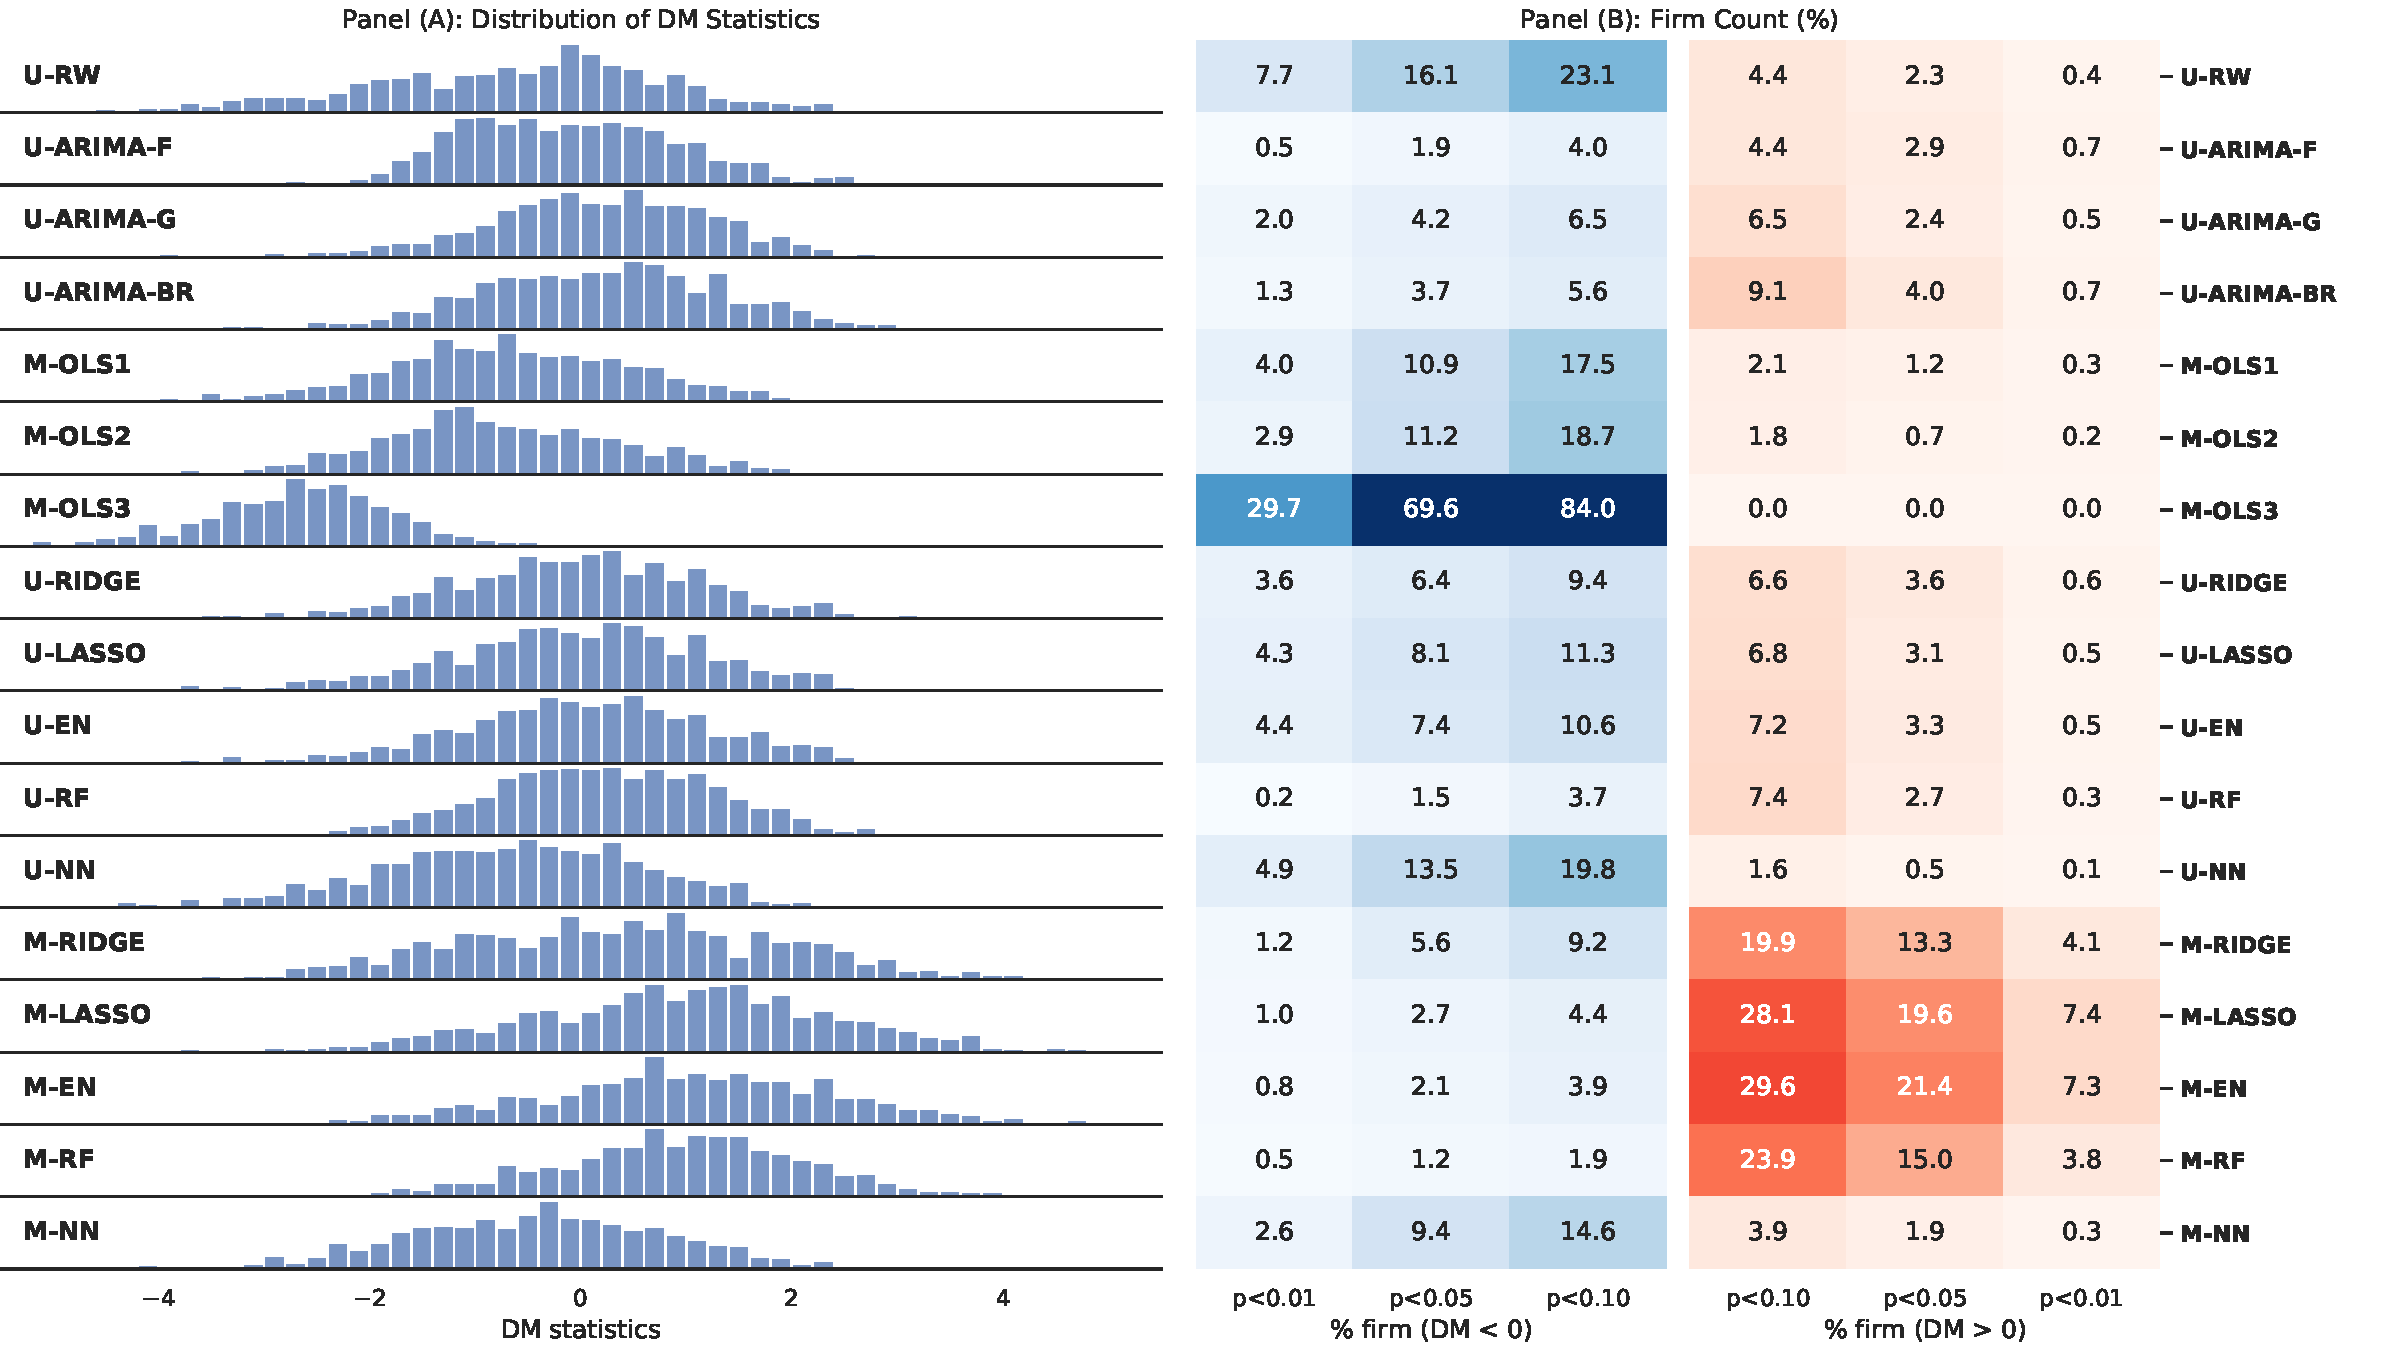
\includegraphics[width=15cm]{./img/_dm_MAD_y_hat_srw.pdf}
  \floatfoot{(注) 各DM検定ではU-SRWをモデル1としており,損失関数はMAEに対応するもの($L(e_t)=|e_t|$)を用いている.Panel(A)はモデル2別の全1,003社のDM統計量の分布をヒストグラムで表している.Panel(B)は全1,003社のDM検定のうち,10\%, 5\%, 1\%の水準で統計的に有意な企業の割合(\%)をDM統計量の正負別に示したヒートマップである.色が濃いほど統計的に有意な企業の割合が大きいことを示している.}
\end{figure}

表\ref{tab:acc}において予測パフォーマンスが最も良いとされる多変量機械学習アルゴリズムが,他の時系列モデルに比べて統計的有意に予測精度が高いかどうかを検定するためにDM検定を行う.まず,ベンチマークモデルと多変量機械学習アルゴリズムの予測精度の差の統計量有意性を検定するために,季節ランダムウォークをモデル1として,その他のモデル全通りをそれぞれモデル2とした場合の両側DM検定を各企業(全1,003社)の予測値系列に対して行う.図\ref{fig:dm_srw}.Panel(A)は全1,003社のDM統計量の分布をモデル2別に示したヒストグラムであり,図\ref{fig:dm_srw}.Panel(B)は全1,003社の両側DM検定のうち,10\%, 5\%, 1\%の水準で統計的に有意な企業の割合(\%)をDM統計量の正負別に示したヒートマップである.なお,図\ref{fig:dm_srw}のDM検定で用いた損失関数はMAEに対応したものである\footnote{MAE以外の精度指標,MAPE, MSPEに対応する損失関数を用いたDM検定も同様な結果であった.}.

図\ref{fig:dm_srw}.Panel(A)より,モデル2が<ーー多変量LASSO回帰,Ridge回帰,Elastic Net回帰,ランダムフォレスト回帰の場合,DM統計量の分布は正の方向に偏っている.ーー>また,図\ref{fig:dm_srw}.Panel(B)から,先述の4つの多変量機械学習アルゴリズムにおいて,<ーーDM統計量が正の値で統計的に有意な企業の割合は,10\%水準の場合約20\%~30\%,5\%水準の場合約13\%~21\%,1\%水準の場合約4\%~7\%となっている.ーー>つまり,多変量Elastic Net回帰と多変量ランダムフォレスト回帰に加え,多変量Ridge回帰と多変量LASSO回帰も,季節ランダムウォークに比べて多くの企業で統計的有意に予測誤差が小さい結果となっており,これは多変量機械学習アルゴリズムが季節ランダムウォークよりも優れた予測を与えていることを意味する.一方,多変量線形回帰モデルについては図\ref{fig:dm_srw}.Panel(A)から<ーーDM統計量の分布は負の方向に偏っておりーー>,図\ref{fig:dm_srw}.Panel(B)でもDM統計量が負の値で統計的に有意な企業の割合が多いことが確認できる.つまり,線形回帰モデルはファンダメンタル会計変数を含めることでかえって予測精度が下がり,予測に何の情報も用いていない季節ランダムウォークよりも劣ってしまうことを意味する.単変量機械学習アルゴリズムについては,図\ref{fig:dm_srw}.Panel(A)と図\ref{fig:dm_srw}.Panel(B)より,統計的有意に予測精度の差がある企業が少なく,季節ランダムウォークと同程度の予測パフォーマンスであることがわかった.

\begin{figure}
  \centering
  \caption{全企業(1,003社)のDM検定結果のまとめ(モデル1: ARIMA-BR, loss: MAE)}
  \label{fig:dm_sarima_br}
  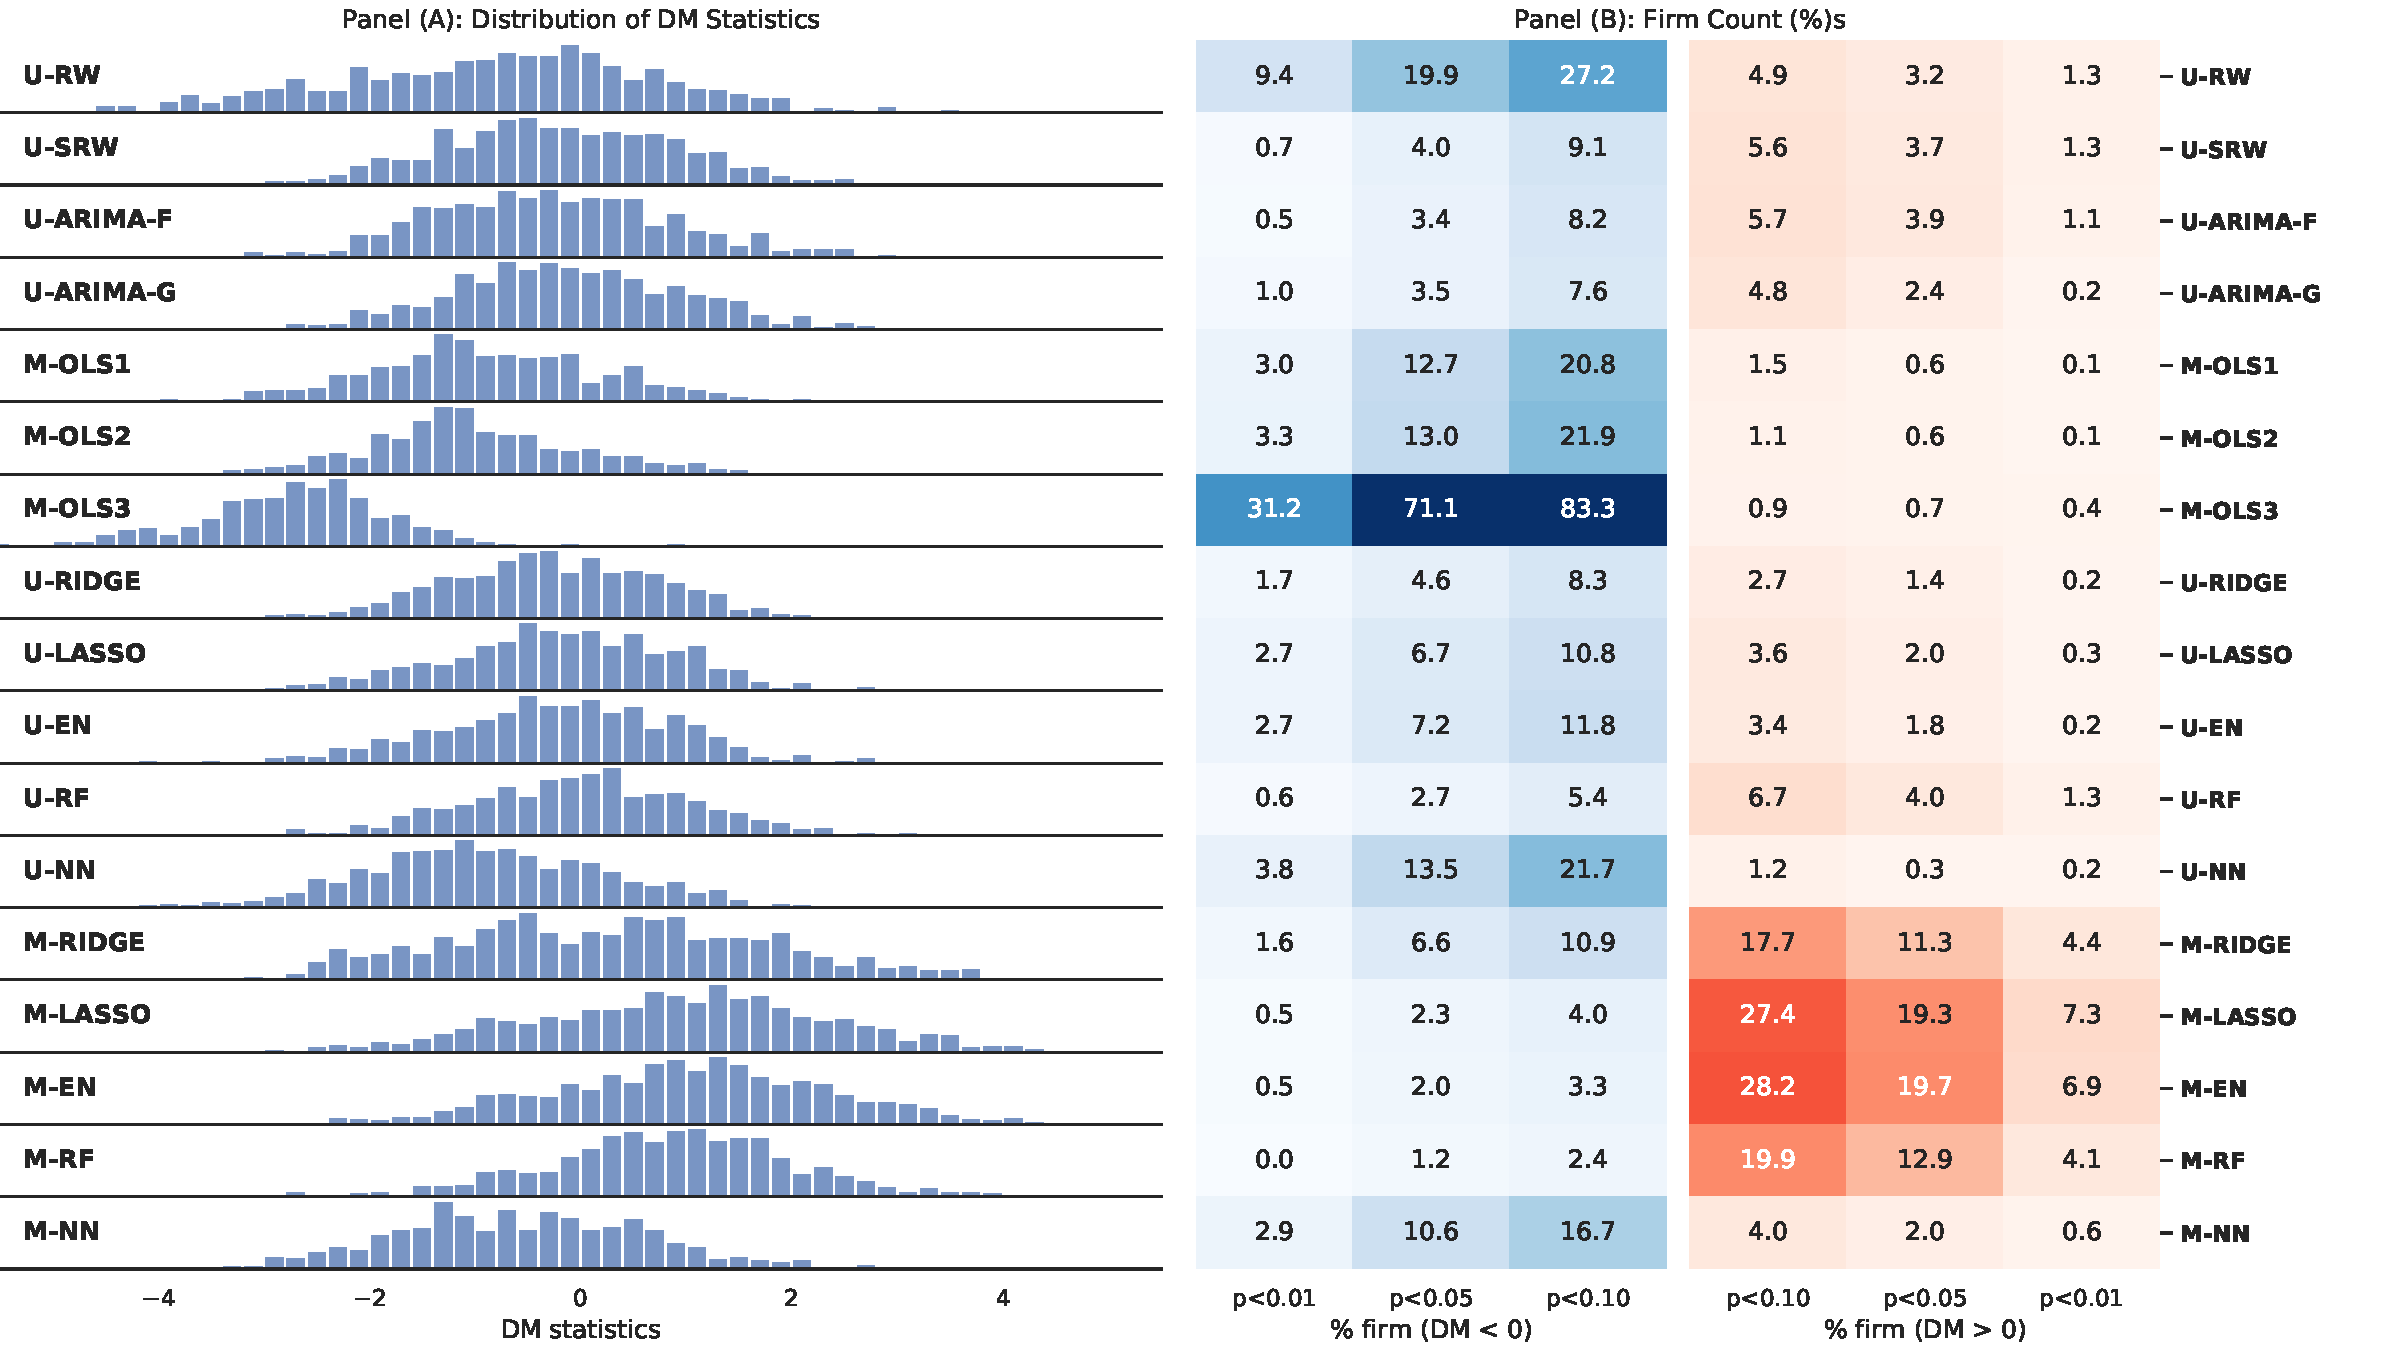
\includegraphics[width=15cm]{./img/_dm_MAD_y_hat_sarima_br.pdf}
  \floatfoot{(注) 各DM検定ではU-ARIMA-BRをモデル1としており,損失関数はMAEに対応するもの($L(e_t)=|e_t|$)を用いている.Panel(A)はモデル2別の全1,003社のDM統計量の分布をヒストグラムで表している.Panel(B)は全1,003社のDM検定のうち,10\%, 5\%, 1\%の水準で統計的に有意な企業の割合(\%)をDM統計量の正負別に示したヒートマップである.色が濃いほど統計的に有意な企業の割合が大きいことを示している.}
\end{figure}

次に,伝統的線形時系列モデルと多変量機械学習アルゴリズムの予測精度の差の統計的有意性を検定するために,\cite{brown1979univariate}のARIMAモデルをモデル1として,その他のモデル全通りをそれぞれモデル2とした場合の両側DM検定を行う.図\ref{fig:dm_sarima_br}.Panel(A)は全1,003社のDM統計量の分布をモデル2別に示したヒストグラムであり,図\ref{fig:dm_sarima_br}.Panel(B)は全1,003社の両側DM検定のうち,10\%, 5\%, 1\%の水準で統計的に有意な企業の割合(\%)をDM統計量の正負別に示したヒートマップである.なお,図\ref{fig:dm_sarima_br}のDM検定で用いた損失関数はMAEに対応したものである\footnote{MAE以外の精度指標,MAPE, MSPEに対応する損失関数を用いたDM検定も同様な結果であった.}.

\cite{brown1979univariate}のARIMAモデルをモデル1としたDM検定の結果は,季節ランダムウォークをモデル1としたDM検定の結果と同様であった.図\ref{fig:dm_sarima_br}.Panel(A)より,モデル2が多変量LASSO回帰,Ridge回帰,Elastic Net回帰,ランダムフォレスト回帰の場合,<ーーDM統計量の分布は正の方向に偏っておりーー>,図\ref{fig:dm_sarima_br}.Panel(B)からもDM統計量が正の値で統計的に有意な企業の割合が多いことが確認できる(10\%,5\%,1\%水準で統計的に有意な企業の割合は,それぞれ約18\%~28\%,11\%~20\%,4\%~7\%).つまり,多変量機械学習アルゴリズムは伝統的な線形時系列モデルである\cite{brown1979univariate}のARIMAモデルよりも多くの企業において統計的有意に予測誤差が小さく,優れた予測を与えていることを意味する\footnote{\cite{foster1977quarterly}, \cite{griffin1977time}のARIMAモデルをそれぞれモデル1としたDM検定も同様な結果であった.}

\section{アナリスト予測との予測精度比較}

本稿では,時系列モデルによる予測と人的な予測の精度を比較するために,人的な予測としてI/B/E/S(Institutional Brokers Estimate System)業績予想を用いる.I/B/E/S業績予想は,複数のアナリストの利益予想の平均値であるコンセンサス予想であり,日本においてもI/B/E/Sの四半期EPS予測がカバーされている企業がある\footnote{全ての上場企業はカバーされていない.}.I/B/E/S業績予想は通常,毎月第3金曜日に更新されており,本稿の時系列モデルの予測タイミングと揃えるために各四半期の中間月末(5月末,8月末,11月末,2月末)時点のI/B/E/S業績予想の1期先四半期EPS予測を比較対象とする.図\ref{fig:ibes_timing}は本稿及びI/B/E/Sの四半期EPS予測のタイミングの概要を表している.

\begin{figure}
  \centering
  \caption{I/B/E/S業績予想の更新タイミング}
  \label{fig:ibes_timing}
  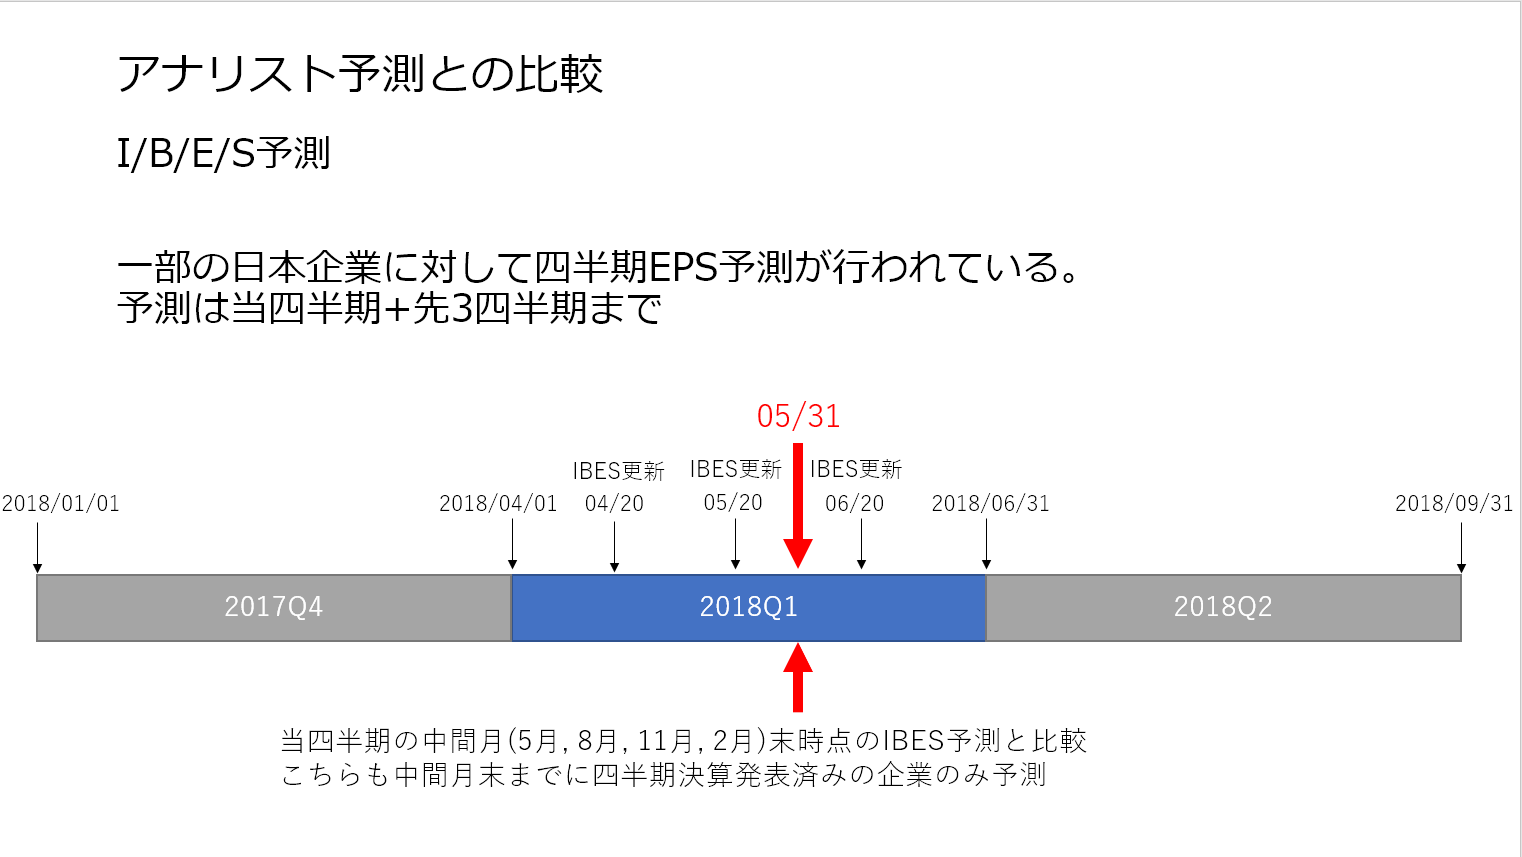
\includegraphics[width=12cm]{./img/_ibes_timing.png}
\end{figure}

本稿で用いるI/B/E/S業績予想のデータは「I/B/E/S on Datastream」から収集している.I/B/E/S業績予想のサンプルについては,第\ref{par:data}部\ref{sec:sample}節と同様な基準のもとで選択し,予測期間についても時系列モデルと同様に2018年度第1四半期~2020年度第4四半期とする.結果として88社,延べ $88社 \times 12四半期 = 1,056個$の企業四半期予測が得られた.なお,時系列モデルとI/B/E/S業績予想の予測精度を比較するために,時系列モデルのサンプル企業については,計算可能であった1,003社からI/B/E/S業績予想が調査対象としている88社に減らして,分析対象企業をI/B/E/S業績予想と揃えることとする.表\ref{tab:acc_ibes}は時系列モデルとI/B/E/S業績予想の,各予測指標の全88社平均を四半期別と全予測期間で集計したものを示している.

\begin{landscape}
\begin{table}
    % \centering
    \caption{時系列モデルによる予測とI/B/E/S業績予想の精度比較(88社平均)}
    \label{tab:acc_ibes}
    \scalebox{0.75}[0.75]{
      %%% threeparttable %%%
\begin{threeparttable}

% \begin{tabular}{lrrrrrrrrrrrrrrrrrrrr}
\begin{tabular}{lrrrp{1.5cm}rrrp{1.5cm}rrrp{1.5cm}rrrp{1.5cm}rrrp{1.5cm}}


\toprule
{} & \multicolumn{4}{c}{Q1} & \multicolumn{4}{c}{Q2} & \multicolumn{4}{c}{Q3} & \multicolumn{4}{c}{Q4} & \multicolumn{4}{c}{Overall} \\
\cmidrule(lr){2-5}
\cmidrule(lr){6-9}
\cmidrule(lr){10-13}
\cmidrule(lr){14-17}
\cmidrule(lr){18-21}
% \tnote
{} &    MAE \tnote{b}&   MAPE \tnote{c}&   MSPE \tnote{d}& Large Forecast Error(\%) \tnote{e}&    MAE &   MAPE &   MSPE & Large Forecast Error(\%) &    MAE &   MAPE &   MSPE & Large Forecast Error(\%) &    MAE &   MAPE &   MSPE & Large Forecast Error(\%) &     MAE &   MAPE &   MSPE & Large Forecast Error(\%) \\
% \tnote
Model \tnote{a}     &        &        &        &                         &        &        &        &                         &        &        &        &                         &        &        &        &                         &         &        &        &                         \\
\midrule
U-RW       &   46.0 &  0.586 &  0.465 &                    29.2 &   31.9 &  0.463 &  0.340 &                    21.6 &   39.7 &  0.443 &  0.317 &                    18.2 &   58.9 &  0.625 &  0.528 &                    37.9 &    44.1 &  0.529 &  0.413 &                    26.7 \\
U-SRW      &   35.9 &  0.491 &  0.372 &                    23.9 &   29.4 &  0.443 &  0.330 &                    22.3 &   41.8 &  0.454 &  0.331 &                    20.5 &   57.4 &  0.602 &  0.496 &                    36.0 &    41.1 &  0.498 &  0.382 &                    25.7 \\
U-ARIMA-F  &   36.6 &  0.487 &  0.374 &                    24.2 &   25.8 &  0.414 &  0.301 &                    19.7 &   41.6 &  0.457 &  0.337 &                    20.8 &   55.6 &  0.602 &  0.490 &                    33.3 &    39.9 &  0.490 &  0.376 &                    24.5 \\
U-ARIMA-G  &   37.2 &  0.522 &  0.405 &                    27.3 &   29.8 &  0.427 &  0.321 &                    21.6 &   41.4 &  0.467 &  0.344 &                    21.6 &   56.5 &  0.607 &  0.498 &                    36.4 &    41.2 &  0.506 &  0.392 &                    26.7 \\
U-ARIMA-BR &   35.8 &  0.498 &  0.380 &                    22.7 &   27.1 &  0.420 &  0.303 &                    18.2 &   36.9 &  0.434 &  0.309 &                    18.2 &   51.3 &  0.583 &  0.471 &                    31.8 &    37.8 &  0.484 &  0.365 &                    22.7 \\
\\
M-OLS1     &   49.7 &  0.574 &  0.458 &                    29.9 &   40.7 &  0.481 &  0.368 &                    26.5 &   46.5 &  0.487 &  0.368 &                    22.7 &   69.0 &  0.597 &  0.486 &                    36.0 &    51.5 &  0.535 &  0.420 &                    28.8 \\
M-OLS2     &   46.9 &  0.550 &  0.438 &                    29.2 &   39.1 &  0.480 &  0.366 &                    24.6 &   85.5 &  0.507 &  0.385 &                    25.4 &   68.1 &  0.641 &  0.548 &                    43.6 &    59.9 &  0.544 &  0.434 &                    30.7 \\
M-OLS3     &  261.9 &  0.777 &  0.712 &                    60.6 &  197.9 &  0.780 &  0.712 &                    59.8 &  207.2 &  0.747 &  0.672 &                    54.9 &  219.0 &  0.780 &  0.714 &                    60.2 &   221.5 &  0.771 &  0.703 &                    58.9 \\
\\
U-RIDGE    &   38.1 &  0.516 &  0.399 &                    26.5 &   31.7 &  0.435 &  0.311 &                    20.8 &   41.7 &  0.463 &  0.334 &                    19.3 &   49.0 &  0.592 &  0.479 &                    34.1 &    40.1 &  0.501 &  0.381 &                    25.2 \\
U-LASSO    &   35.2 &  0.529 &  0.403 &                    24.2 &   28.1 &  0.431 &  0.296 &                    16.7 &   38.5 &  0.471 &  0.335 &                    17.0 &   44.9 &  0.587 &  0.468 &                    31.8 &    36.7 &  0.504 &  0.376 &                    22.4 \\
U-EN       &   34.9 &  0.522 &  0.395 &                    23.9 &   27.7 &  0.424 &  0.292 &                    16.3 &   38.2 &  0.466 &  0.327 &                    15.9 &   44.6 &  0.584 &  0.465 &                    31.1 &    36.3 &  0.499 &  0.370 &                    21.8 \\
U-RF       &   34.2 &  0.510 &  0.389 &                    26.1 &   28.7 &  0.413 &  0.283 &                    17.4 &   38.6 &  0.460 &  0.322 &                    17.0 &   46.9 &  0.568 &  0.451 &                    30.7 &    37.1 &  0.488 &  0.361 &                    22.8 \\
U-NN       &   43.3 &  0.581 &  0.458 &                    27.3 &   35.8 &  0.507 &  0.375 &                    22.0 &   43.5 &  0.508 &  0.373 &                    20.8 &   54.0 &  0.635 &  0.525 &                    35.2 &    44.2 &  0.558 &  0.433 &                    26.3 \\
\\
M-RIDGE    &   48.2 &  0.509 &  0.402 &                    28.0 &   41.9 &  0.490 &  0.379 &                    25.4 &   44.9 &  0.461 &  0.346 &                    22.3 &   54.3 &  0.551 &  0.457 &                    34.1 &    47.3 &  0.503 &  0.396 &                    27.5 \\
M-LASSO    &   25.0 &  0.432 &  0.315 &                    18.6 &   22.4 &  0.389 &  0.263 &                    13.6 &   30.7 &  0.391 &  0.276 &                    17.4 &   36.6 &  0.488 &  0.378 &                    26.1 &    28.7 &  0.425 &  0.308 &                    18.9 \\
M-EN       &   25.8 &  0.426 &  0.310 &                    18.2 &   24.0 &  0.404 &  0.277 &                    14.8 &   31.3 &  0.407 &  0.291 &                    17.8 &   39.4 &  0.501 &  0.392 &                    27.7 &    30.1 &  0.435 &  0.318 &                    19.6 \\
M-RF       &   26.3 &  0.439 &  0.320 &                    19.7 &   22.6 &  0.375 &  0.262 &                    17.4 &   34.1 &  0.396 &  0.275 &                    18.2 &   40.2 &  0.526 &  0.410 &                    28.8 &    30.8 &  0.434 &  0.317 &                    21.0 \\
M-NN       &   41.0 &  0.536 &  0.414 &                    28.0 &   36.1 &  0.505 &  0.381 &                    25.0 &   41.3 &  0.483 &  0.355 &                    20.5 &   54.1 &  0.606 &  0.493 &                    33.0 &    43.1 &  0.532 &  0.411 &                    26.6 \\
\\
IBES       &   29.1 &  0.426 &  0.298 &                    15.9 &   26.8 &  0.390 &  0.262 &                    13.6 &   33.1 &  0.385 &  0.253 &                    12.9 &   37.1 &  0.479 &  0.364 &                    25.0 &    31.5 &  0.420 &  0.294 &                    16.9 \\
\\
\# of Forecasts     & \multicolumn{4}{c}{N=264} & \multicolumn{4}{c}{N=264} & \multicolumn{4}{c}{N=264} & \multicolumn{4}{c}{N=264} & \multicolumn{4}{c}{N=1,056} \\
\bottomrule
\end{tabular}

%%% table footnote %%%
\begin{tablenotes}
\item[a] 各モデルの先頭文字列U-は単変量モデル,M-は多変量モデルを表す. また,RWはランダムウオーク,SRWは季節ランダムウオーク,ARIMA-F,ARIMA-G,ARIMA-BRはそれぞれ\cite*{foster1977quarterly, griffin1977time, brown1979univariate}の設定のARIMAモデル,OLS1,OLS2,OLS3はそれぞれ式(\ref{eq:ols1}),式(\ref{eq:ols2}),式(\ref{eq:ols3})の線形回帰モデル,RIDGEはRidge回帰,LASSOはLASSO回帰,ENはElastic Net回帰,RFはランダムフォレスト回帰,NNはニューラルネットワークを表す.IBESはI/B/E/S業績予想を表す.
\item[b] 平均絶対誤差(Mean Absolute Error: MAE)
\item[c] 平均絶対誤差率(Mean Absolute Percentage Error: MAPE)
\item[d] 平均二乗誤差率(Mean Squared Percentage Error: MSPE)
\item[e] 絶対予測誤差率$\left| \frac{Y_t -{\hat Y}_t}{Y_t} \right|$が1を超えるLarge Forecast Errorサンプルについては絶対予測誤差率を1としており,全予測サンプルに占めるLarge Forecast Errorサンプルの割合(\%)を示している.
\item[] (出所)筆者作成. 
\end{tablenotes}
\end{threeparttable}
    }
\end{table}
\end{landscape}

全予測期間平均でMAEが最小のモデルは多変量LASSO回帰(28.7),次いで多変量Elastic Net回帰(30.1),ランダムフォレスト回帰(30.8)となり,多変量機械学習アルゴリズムがアナリスト予測であるI/B/E/S業績予想のMAE(31.5)を下回った.一方で,他の予測精度指標ではいずれもI/B/E/S業績予想が最も小さい値となり(MAPE, MSPE, Large Forecast Errorがそれぞれ0.420,0.294,16.9\%),多変量機械学習アルゴリズム(特にLASSO回帰,Elastic Net回帰,ランダムフォレスト回帰)はI/B/E/S業績予想と比較するとわずかに予測精度が低い結果となった.各四半期別平均についても同様な傾向が見られ,MAEにおいては機械学習アルゴリズムの方がI/B/E/S業績予想よりも予測精度が高いものの,他の予測精度指標ではI/B/E/S業績予想よりも予測精度が低い結果となった.

% 森(1998)は半期予測でサンプルも3社ではあるものの,伝統的時系列モデルがアナリストと遜色ない結果
% いままでの暗黙の了解とは異なる結果.
% IBESのほうがいい --> アナリストは時系列モデルで利用しファンダメンタル会計変数以外にも多くの情報を織り込んでいる.--> にもかかわらず

なお,表\ref{tab:acc}と表\ref{tab:acc_ibes}を比較すると,時系列モデルでは,もともと計算可能な1,003社平均よりもI/B/E/S業績予想が調査対象としている88社平均のほうが全体的に精度が高い傾向がみられる.<ーーそもそもアナリストは全ての上場企業をカバーしているわけではなく,限られた企業のみを調査対象としているのが日本の現状である.これについて\cite{nakai2006}は,アナリストは情報が入手しやすい企業をカバーする傾向にあると指摘しており,I/B/E/S業績予想のアナリストの調査対象企業は比較的に予測が容易である可能性が示唆される.ーー>
% 投資機会の拡張,平等な投資機会という意味でも時系列モデルはいいのでは? 米山(2010)

\section{アナリスト予測との予測精度差の検定}

\begin{figure}
  \centering
  \caption{全企業(88社)のDM検定結果のまとめ(モデル1: IBES, loss: MAE)}
  \label{fig:dm_ibes_mad}
  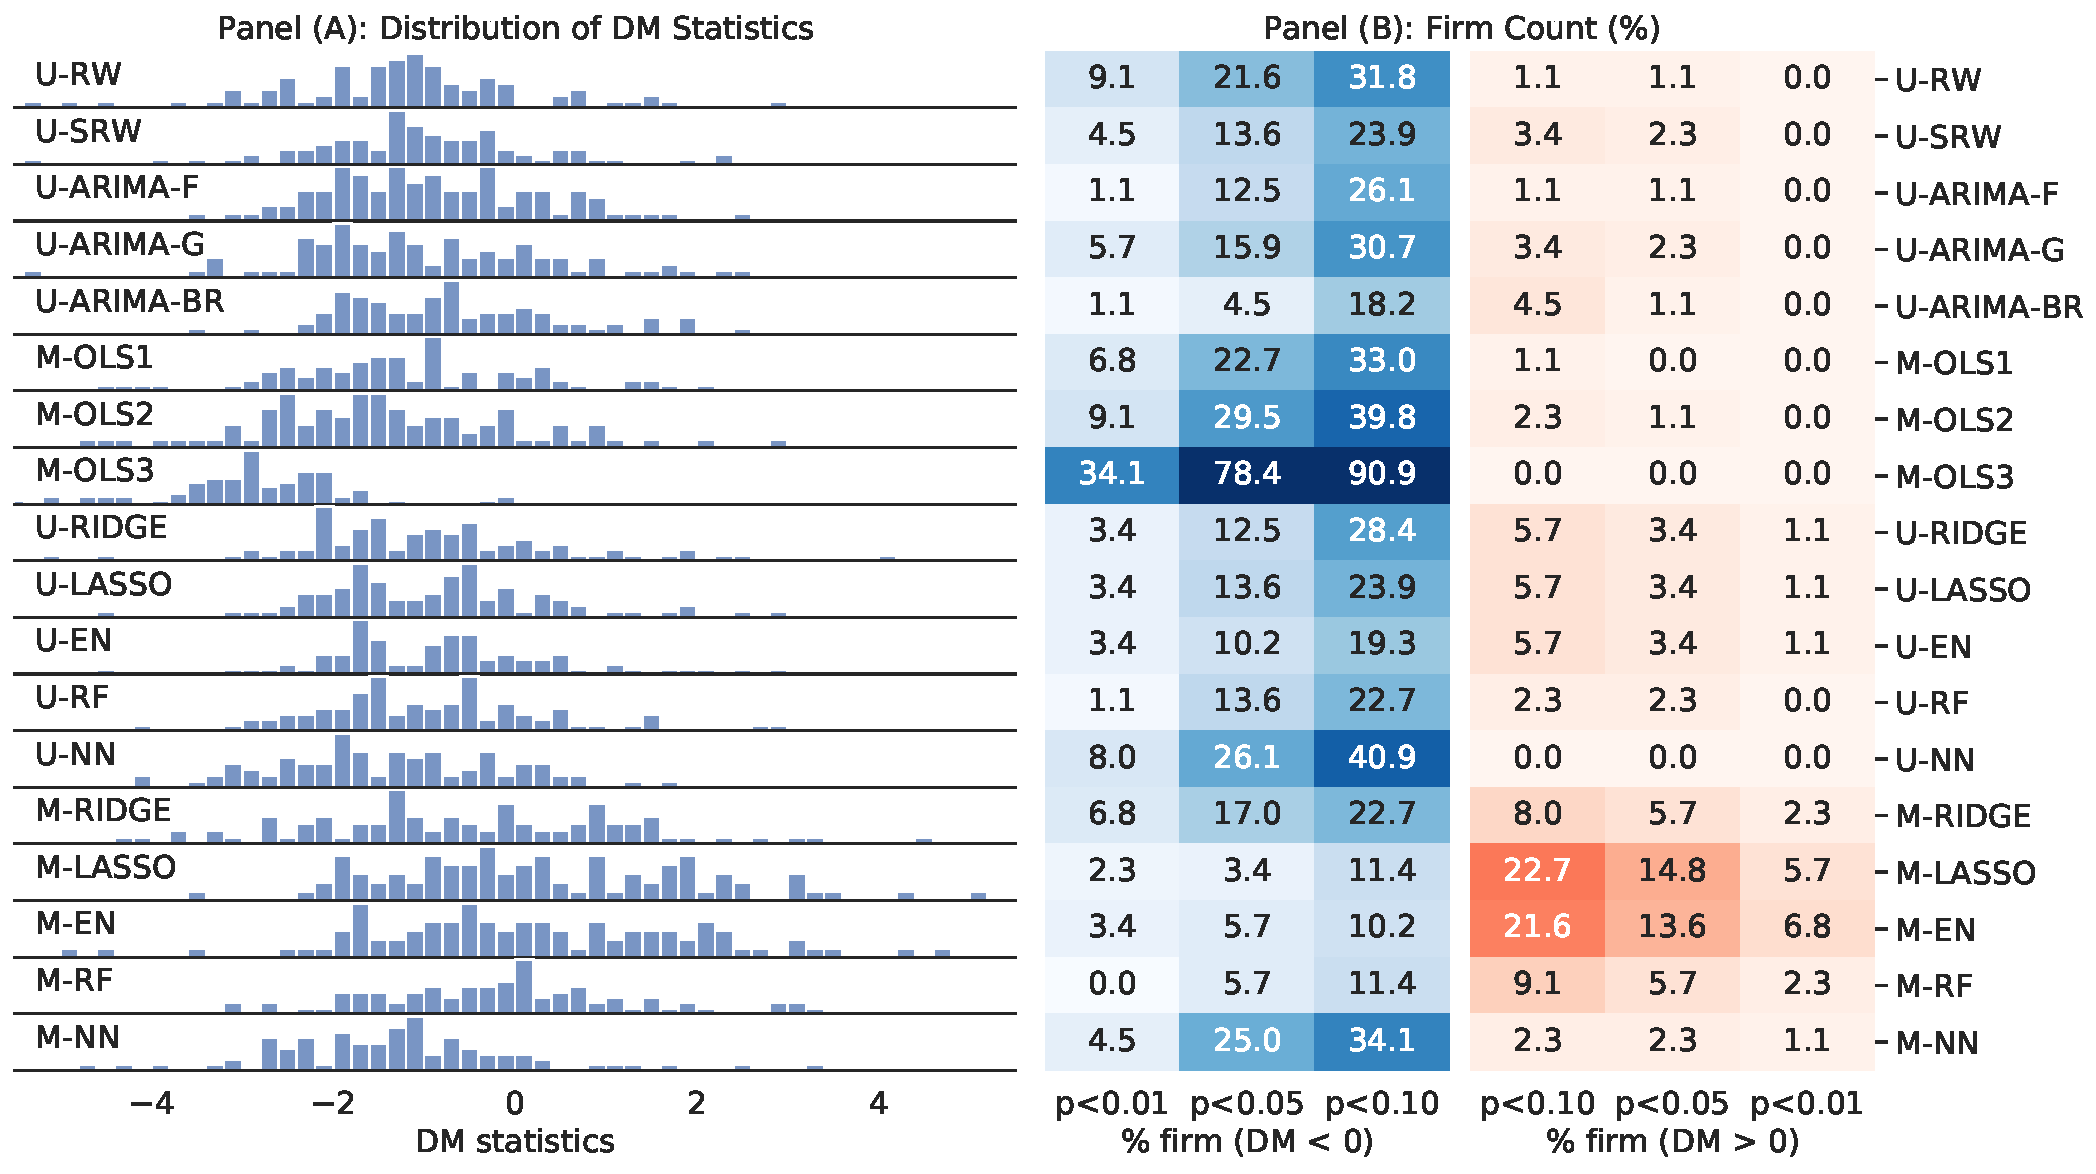
\includegraphics[width=15cm]{./img/_dm_MAD_y_hat_ibes.pdf}
  \floatfoot{(注) 各DM検定ではIBESをモデル1としており,損失関数はMAEに対応するもの($L(e_t)=|e_t|$)を用いている.Panel(A)はモデル2別の全88社のDM統計量の分布をヒストグラムで表している.Panel(B)は全88社のDM検定のうち,10\%, 5\%, 1\%の水準で統計的に有意な企業の割合(\%)をDM統計量の正負別に示したヒートマップである.色が濃いほど統計的に有意な企業の割合が大きいことを示している.}
\end{figure}

まず,表\ref{tab:acc_ibes}でMAEがI/B/E/S業績予想よりも小さい多変量LASSO回帰,Elastic Net回帰,ランダムフォレスト回帰が,I/B/E/S業績予想と比べて統計的有意に予測誤差が小さいかどうかをDM検定する.具体的にはI/B/E/S業績予想をモデル1として,その他のモデル全通りをそれぞれモデル2とした場合の,損失関数をMAEに対応するものとした両側DM検定を,I/B/E/S業績予想が調査の対象としている企業(全88社)の予測値系列に対して行う.図\ref{fig:dm_ibes_mad}.Panel(A)は全88社のDM統計量の分布をモデル2別に示したヒストグラムであり,図\ref{fig:dm_ibes_mad}.Panel(B)は全88社の両側DM検定のうち,10\%, 5\%, 1\%の水準で統計的に有意な企業の割合(\%)をDM統計量の正負別に示したヒートマップである.

図\ref{fig:dm_ibes_mad}.Panel(A)より,多くの時系列モデル(特に単変量線形時系列モデル,多変量線形回帰モデル,単変量機械学習アルゴリズム)で<ーーDM統計量の分布が負の方向に偏っている.ーー>図\ref{fig:dm_ibes_mad}.Panel(B)でも多くの時系列モデルにおいてDM統計量が負の値で統計的に有意な企業の割合が多いことが確認でき,アナリスト予測は単変量線形時系列モデル,多変量線形回帰モデル,単変量機械学習アルゴリズムによる予測よりも精度が高いことを示している.一方,I/B/E/S業績予想と多変量械学習アルゴリズムの検定結果では,図\ref{fig:dm_ibes_mad}.Panel(A)より,モデル2が多変量LASSO回帰とElastic Net回帰のとき<ーーDM検定量の分布が正の方向に偏っておりーー>,図\ref{fig:dm_ibes_mad}.Panel(B)から,DM統計量が正の値で統計的に有意な企業の割合が多いことが確認できる(10\%,5\%,1\%水準で統計的に有意な企業の割合は,それぞれ約22~23\%,14~15\%,6~7\%).つまり,MAEにおいて多変量機械学習アルゴリズムはアナリスト予測であるI/B/E/S業績予想よりも多くの企業において統計的有意に予測誤差が小さく,優れた予測を与えていることを意味する.なお,モデル2が多変量ランダムフォレスト回帰の場合は有意水準と統計的有意に異なった企業の割合が同程度であり,I/B/E/S業績予想と多変量ランダムフォレスト回帰の予測精度に差はない結果となった.

\begin{figure}
  \centering
  \caption{全企業(88社)のDM検定結果のまとめ(モデル1: IBES, loss: MAPE)}
  \label{fig:dm_ibes_mape}
  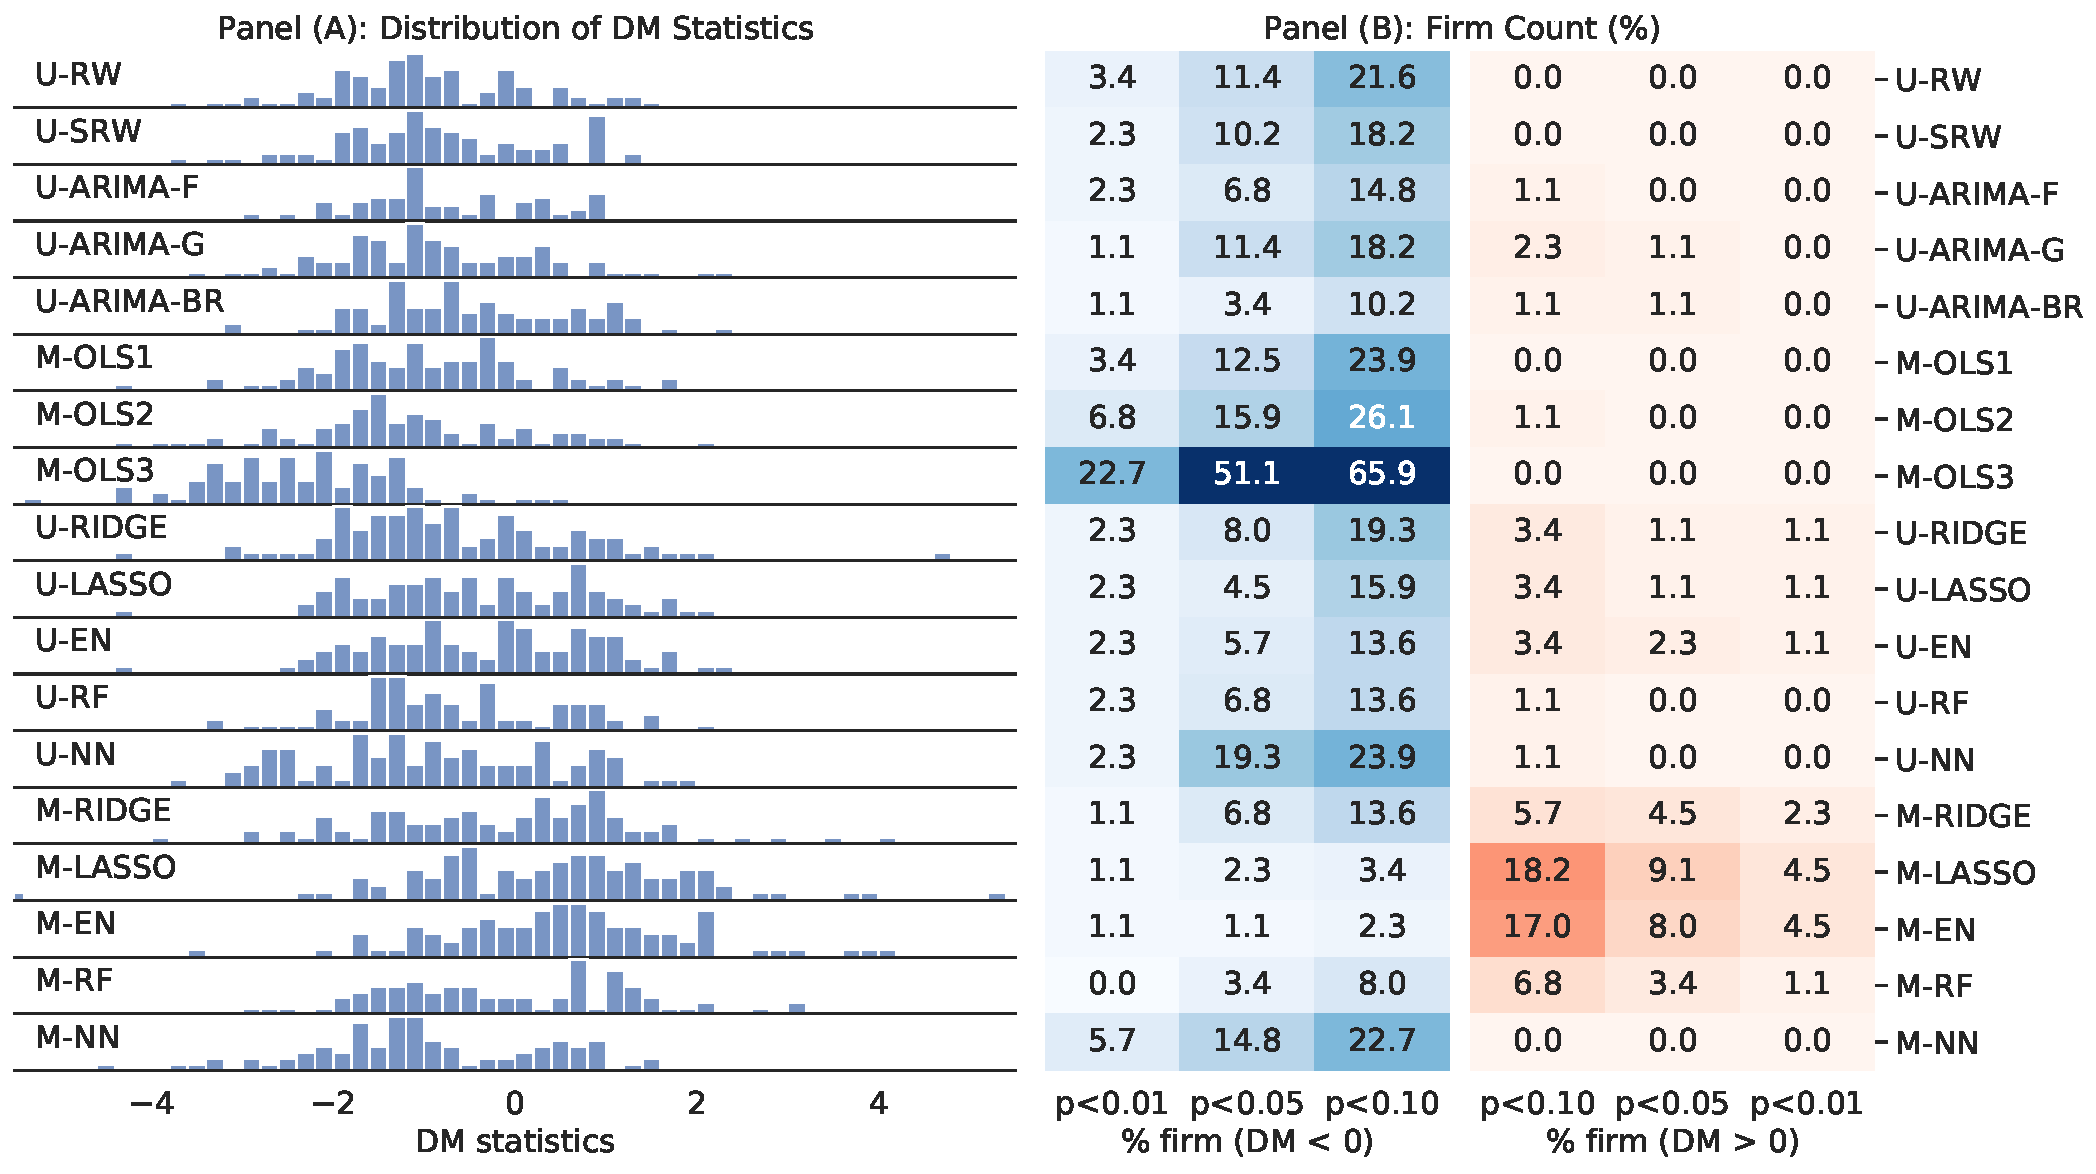
\includegraphics[width=15cm]{./img/_dm_MAPE_y_hat_ibes.pdf}
  \floatfoot{(注) 各DM検定ではIBESをモデル1としており,損失関数はMAEに対応するもの($L(e_t)=\left|\frac{e_t}{Y_t}\right|$)を用いている.Panel(A)はモデル2別の全88社のDM統計量の分布をヒストグラムで表している.Panel(B)は全88社のDM検定のうち,10\%, 5\%, 1\%の水準で統計的に有意な企業の割合(\%)をDM統計量の正負別に示したヒートマップである.色が濃いほど統計的に有意な企業の割合が大きいことを示している.}
\end{figure}

次に,損失関数をMAPEに対応するものとした両側DM検定を行い,図\ref{fig:dm_ibes_mape}にその結果をまとめている.表\ref{tab:acc_ibes}ではI/B/E/S業績予想と多変量機械学習アルゴリズムをMAPEで比較すると,I/B/E/S業績予想の方が小さい値であったが,図\ref{fig:dm_ibes_mape}.Panel(A)より,モデル2が多変量LASSO回帰とElastic Net回帰のとき<ーーDM統計量が正の方向に偏っておりーー>,図\ref{fig:dm_ibes_mape}.Panel(B)から,DM統計量が正の値で統計的に有意な企業の割合が多いことも確認できる(10\%,5\%,1\%水準で統計的に有意な企業の割合は,それぞれ約17~18\%,8~9\%,5\%).また,モデル2が多変量ランダムフォレスト回帰の場合はI/B/E/S業績予想と同程度の精度の予測を与えている.なお,損失関数をMSPEに対応するものとした両側DM検定でも同様な結果が得られ,多変量機械学習アルゴリズムはアナリスト予測と比べると統計的有意に精度が高い,もしくは精度の差がない予測を与える企業が多い結果となった.

通常,アナリストは本稿の時系列モデルが用いる情報(過去の四半期EPSの実績値や過去のファンダメンタル会計変数)以外にも広範囲の情報を反映した予測を行うと考えられるため\citep{sakurai1990},アナリスト予測は(多変量機械学習アルゴリズムも含めた)時系列モデルによる予測よりも精度が高いとされる.にもかかわらず本稿のDM検定の結果から,多変量機械学習アルゴリズムはアナリスト予測と同等もしくはそれ以上に高い精度の予測を与えることが示された.

\part{予測の投資指標としての有用性} \label{par:portfolio}

最後に,本稿で推定した機械学習アルゴリズムによって得られた1期先四半期EPS予測の投資指標としての有用性について検証する.検証方法としては,代表的な投資指標である株価収益率を1期先四半期EPS予測値をもとに算出し,得られた株価予測収益率の高低によってロング・ショート・ポートフォリオを構築してどれくらいの超過リターンが得られるかを調べる.具体的には次のように行う.

\begin{enumerate}
  \item 時点$t-1$(各四半期の中間月末)において,株価$P_{t-1}$と1期先四半期EPS予測値$\hat{Y}_t$を用いて株価予測収益率$\frac{P_{t-1}}{\hat{Y}_t}$を全企業に対して計算する.
  % 現在の時点をtとすれば,1期先予測はt+1.でもモデルの表記と揃えるか.
  \item 全サンプル企業(時系列モデルは全1,003社,I/B/E/S業績予想は全88社)の株価予測収益率を降順にソートし,倍率順に1~5までの5つのポートフォリオを作成する.
  \item 高倍率企業で構成されるポートフォリオ1を空売りし,低倍率企業で構成されるポートフォリオ5を同じ額だけ買う.
  \item 1四半期(3ヶ月)保有し,ポートフォリオ1とポートフォリオ5のスプレッドを観測する.
\end{enumerate}

以上のような操作を毎四半期行い,ポートフォリオを1四半期ごとにリバランスする.図\ref{fig:portfolio_return}は各予測手法に基づくロング・ショート・ポートフォリオ戦略の累積超過リターンを2018年5月末~2021年2月末まで示している.

\begin{figure}
  \centering
  \caption{各予測手法に基づいたロング・ショート・ポートフォリオ戦略による累積超過リターン}
  \label{fig:portfolio_return}
  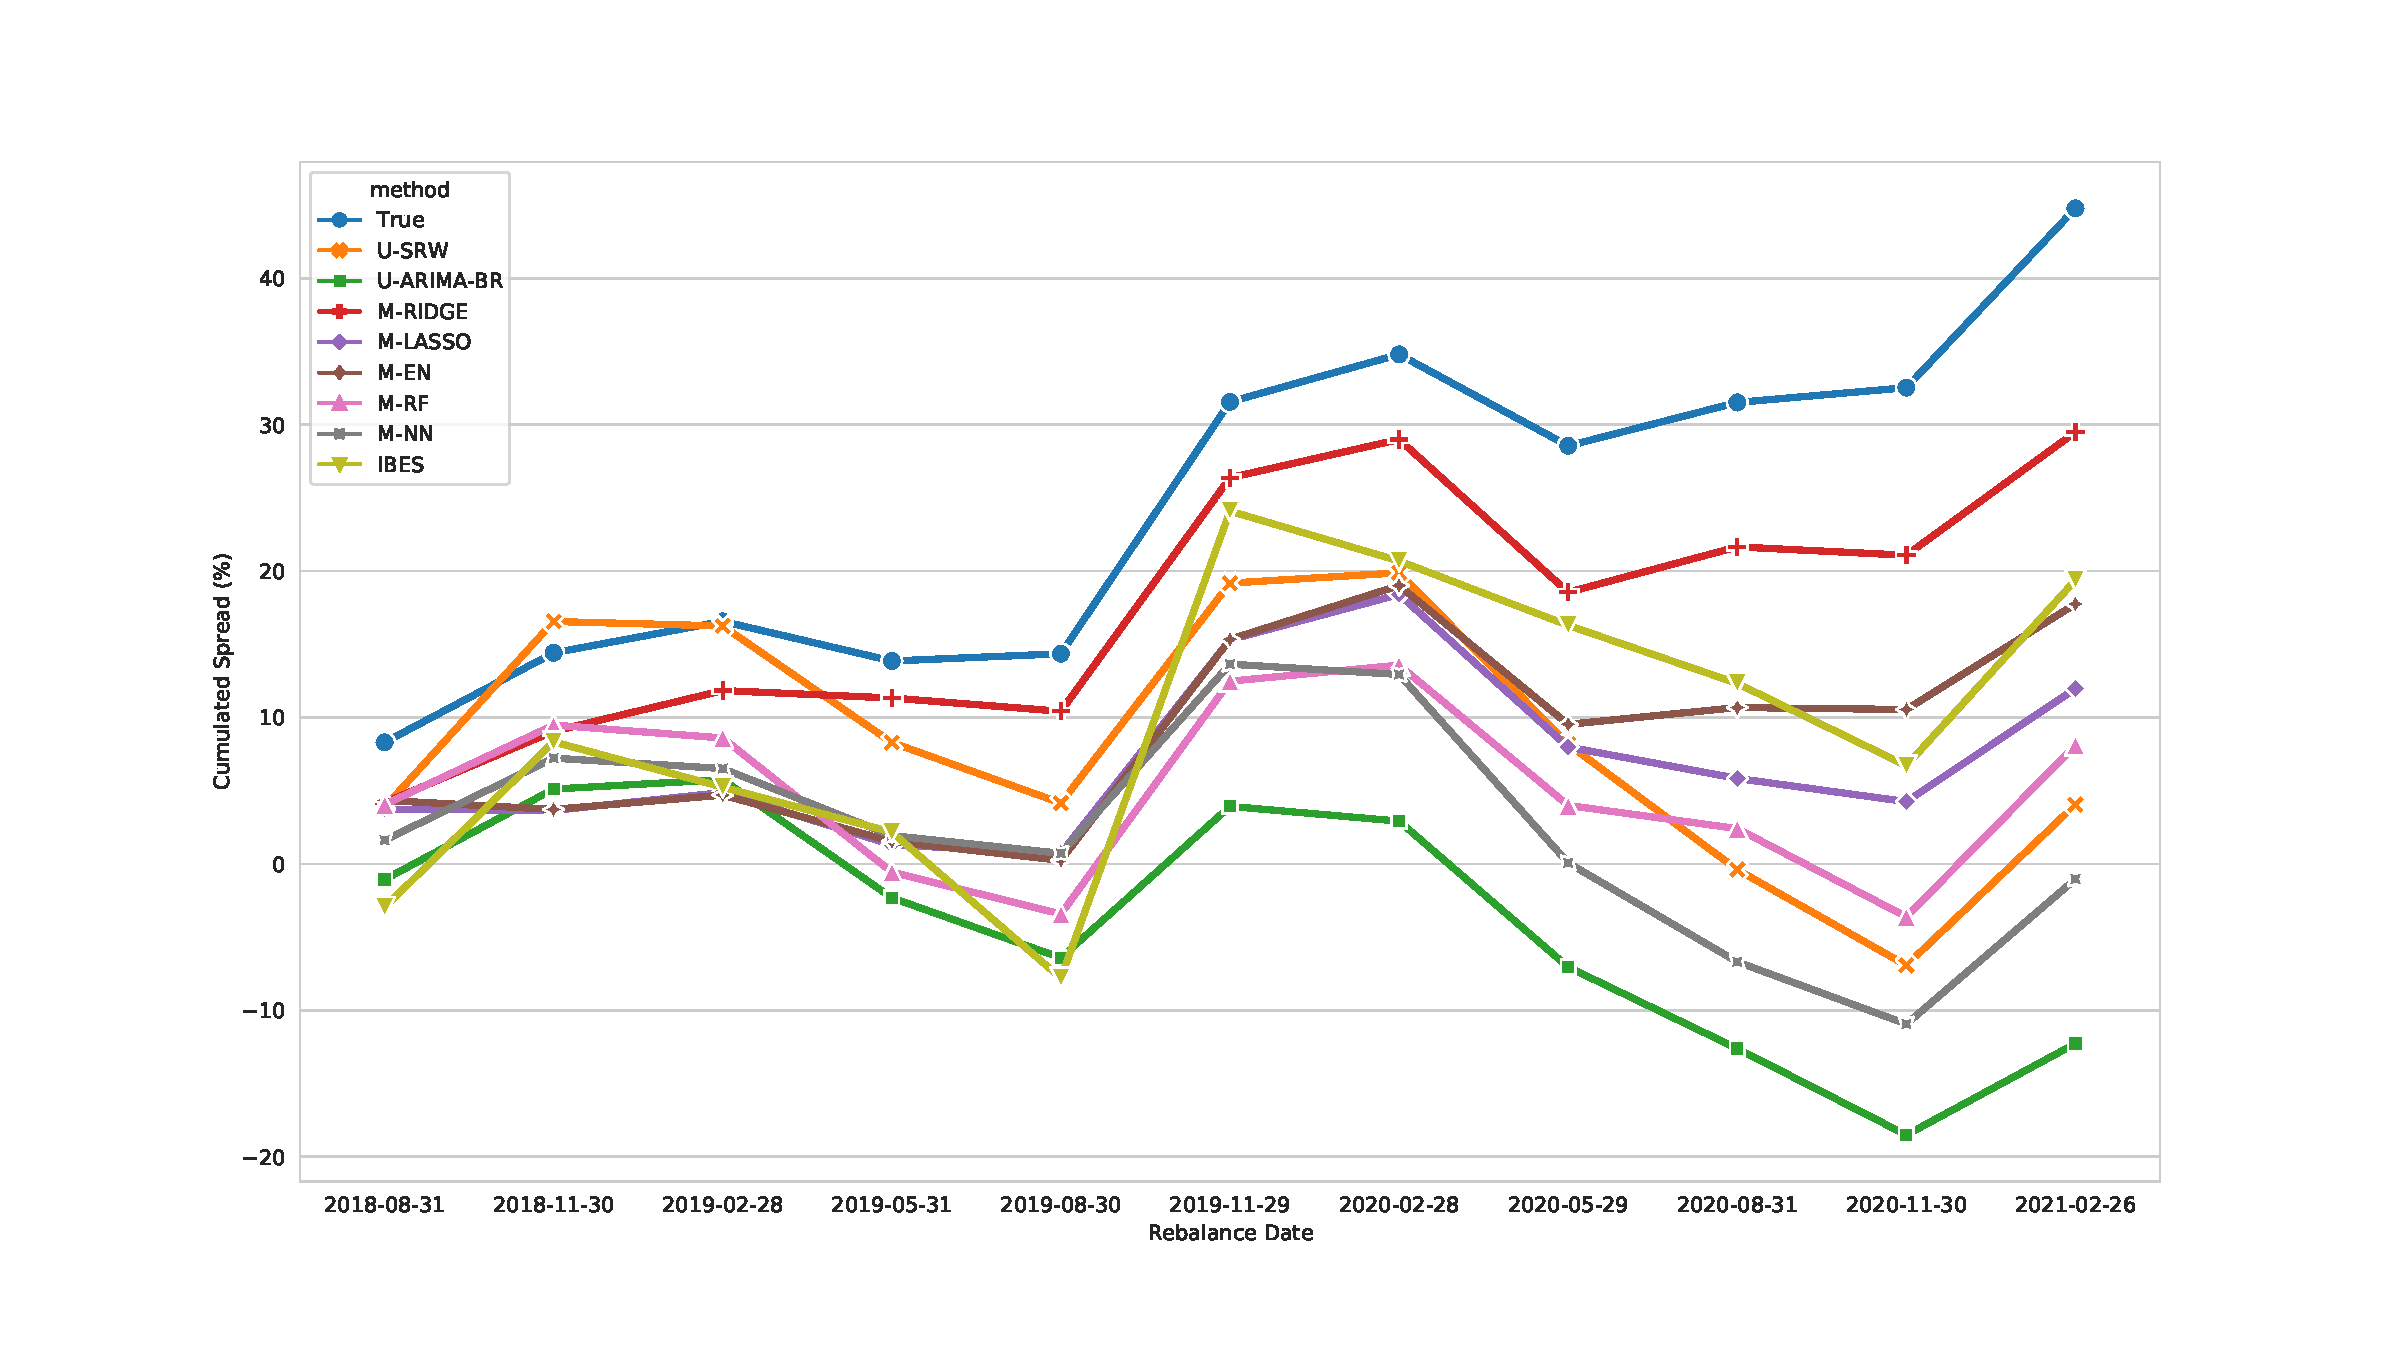
\includegraphics[width=15cm]{./img/_portfolio_return.pdf}
  \floatfoot{(注) リターン算出に用いた株価データは「日経NEEDS-FinancialQUEST」から収集している.Trueは株価予測収益率の算出に1期先四半期EPSの真の値を用いたときの超過リターンを示している.季節ランダムウオークモデル(U-SRW)は1年前の実績四半期EPSを用いた株価予測収益率を算出しているとみなすことができる.なお,株価予測収益率が負である企業は除外してポートフォリオを構築している.}
\end{figure}

まず,1期先四半期EPSの真の値をロング・ショート・ポートフォリオ戦略に用いると,プラスのリターンを獲得している.つまり,仮に1期前時点で次期四半期EPSを完璧に予測できるのであれば高い水準の超過リターンを得ることができることを意味する.各予測手法のうち,最も高いリターンを獲得したのは多変量Ridge回帰であり,最終時点の累積超過リターンは約30\%となった.次点でI/B/E/S業績予想が高いリターンを得ており,多変量Elastic Net回帰がそれをわずかに下回る結果となった.ここで,I/B/E/S業績予想の超過リターンの標準偏差は12.2であり,他の時系列モデルの超過リターンの標準偏差(平均7.1)と比べると変動が大きいことがわかる.これは時系列モデルのサンプル企業が1,003社であるのに対し,I/B/E/S業績予想のカバレッジが88社と少数であるためリターンの変動が大きくなっていると考えられる.なお,伝統的な線形時系列モデル(季節ランダムウオークモデル,\cite{brown1979univariate}のARIMAモデル)の超過リターンはいずれも低い水準の超過リターンであった.このように,機械学習アルゴリズム(特に多変量Ridge回帰)による予測には投資指標における有用性があることが確認された.

\part{終わりに} \label{par:conclusion}

本稿では,機械学習アルゴリズムによる日本企業の四半期EPS予測を行い,伝統的な線形時系列モデルとの精度比較と,アナリスト予測との精度比較をそれぞれ行った.まず,伝統的な線形時系列モデルとの比較について,単変量予測ではあまり予測精度の差は見られなかったものの,多変量予測では機械学習アルゴリズムが明らかに伝統的な線形時系列モデルよりも精度の高い予測を与えた.この結果から,機械学習アルゴリズムは伝統的な線形時系列モデルでは捉えられない将来の四半期EPSとファンダメンタル会計変数の関係性を捉えることができ,機械学習アルゴリズムを用いることで統計的・機械的な手法による日本企業のEPS予測のパフォーマンスを向上させる可能性が示唆される.次に,アナリスト予測との比較について,多変量機械学習アルゴリズムはアナリスト予測と同等もしくはそれ以上に高い精度の予測を与えた.企業利益予測の研究分野では,長らく時系列モデルによる予測よりもアナリスト予測の方が適切であると暗黙裡に見なされてきたが,本稿の結果はその認識を覆すものとなった.さらに本稿の追加的な検証から,機械学習アルゴリズムによる四半期EPS予測値は投資指標としても優れており,多くの企業を予測対象とすることでより分散の効いた投資機会を得ることができると考えられる.

機械学習アルゴリズムがアナリストと同等な精度の予測を与えることに加え,統計的・機械的な手法である機械学習アルゴリズムは予測プロセスが自動化されているため低コストであり,かつ決算情報を公開する企業であれば全て予測対象とすることができる.\cite{yoneyama2010}によると日本企業のアナリストカバレッジは減少している傾向にあり,特に新興市場のカバー率は全体で10\%に満たないものとなっている.日本証券業協会はこうした事態に対処するため,「アナリストの中立性に配慮しつつ、新興市場に上場する企業のアナリストカバレッジを高める施策を検討する」という提言を行った\footnote{日本証券業協会「新興市場のあり方を考える委員会報告書」参照.}.しかし現実の問題としてアナリストは,重要顧客である機関投資家の保有比率が高く,株式売買が盛んで,売買手数料が大きい企業のみをカバーする傾向にあり\citep{nakai2006},市場で株式売買が少ない企業にアナリストの関心を引きつけることは困難で,費用対効果の問題も伴う.このような日本のアナリスト予測のカバレッジが限定的である現状に対し,機械学習アルゴリズムを用いることで,アナリストの関心を引かないような企業に対してもアナリストと同等もしくはそれ以上の精度の利益予測を低コストで提供できるであろう.

本稿の課題として,まず予測をより早い時点で実行できるようにすることが考えられる.本稿の予測のデザインは,前期四半期決算情報の開示後,その情報をもとに1期先四半期EPSを予測するものとなっている.一方で,2期先,3期先のようにより早い時点で予測を行うことも十分に考えらる.その場合,予測に用いることができる情報集合を予測タイミング時点で利用可能なものに限定したうえで,複数期先予測の精度が保たれるのかを検証することが必要となるであろう.次に,過去の四半期EPSの実績値やファンダメンタル会計変数以外にも予測に用いることができる情報があるのかどうかを吟味することも挙げられる.本稿の予測で用いた説明変数は,公開された対象企業自身の会計データに限定しており,1企業内で完結しているものとなっている.しかし,企業の将来の利益を説明するものとして,マクロ要因や産業別要因,利害関係がある企業の情報なども考えられる.そのような対象企業外の情報の中から予測精度を向上させるものを模索することも有意義であろう.

機械学習アルゴリズムはハイパーパラメータ選択のプロセスやモデルの設定によって予測のパフォーマンスが大きく変動するため,本稿で得られた結果は必ずしも最良なものではないかもしれない.それでも本稿の結果はアナリストと比べて劣らない,もしくは優れた予測を与えるものとなった.このことから,現在日本で衰退してしまっている時系列モデルによる利益予測の研究が,機械学習アルゴリズムを用いることで再興する余地が十分にあることが示唆される.今後の研究で,統計的・機械的な手法による企業利益予測を更に発展させ,あらゆるステークホルダーに利用可能な幅広い企業の予測情報が提供されることを期待したい.

% 森(1998)の会計の話を少し入れるか

% 多変量機械学習モデルは,,,,
% * 伝統的な単変量線形モデルよりもいい.優れた予測
% * アナリストとはどっこいどっこい.検定すればむしろ勝ち.
% * アナリストのカバーは少ないしコスト高い.統計機械モデルはデータがあればどんな企業でもできるし0円
% --> アナリストカバレッジの偏りの是正

% このことから,今まで暗黙裡に人>モデルは誤っていることが考えられる.
% アナリストカバレッジは小さい.コストがかからない自動化された統計的・機械的な時系列モデルによる予測を「市場の期待利益」として用いることが妥当である可能性がある.
% これを機に日本でも機械学習アルゴリズムを用いた企業利益の時系列予測に関する研究が発展することを願う.

% future research
% より早い時点で(これは,n期先予測もさせることを意味する)
% 説明変数の増加 (マクロ経済変数とか)させて予測精度の向上(本稿では企業の決算情報に限定し,1企業で完結させたが)
% NNの発展させたもの(num hidden layerの追加LSTMとか?)

% 本稿の図表は全て筆者作成
% githubソースコード

% https://www.eng.u-hyogo.ac.jp/faculty/hoshino/pc/tex_bibtex/
% http://mikilab.doshisha.ac.jp/dia/seminar/latex/doc/bib.html
% Harvard style
% \bibliographystyle{agsm}
%%% BibTeX スタイルファイルの指定.jecon.bst を指定.
\bibliographystyle{jecon}
% \bibliographystyle{jplain}
\bibliography{ref}

\appendix 

% DMtestのヒストグラム.精度の差がないモデル同士もやってplacebo test
% 載せたつの,全通りマトリクスver
% MAPE, MSPEのDM検定結果
% 時系列プロット?

\end{document}
